\documentclass[11pt,a4paper]{article}
\usepackage [latin1]{inputenc}
\usepackage{amsthm}
\usepackage{amsfonts}
\usepackage{geometry}
\usepackage{amsmath}
\usepackage{multirow, makecell}
\usepackage{amssymb}
\usepackage{graphicx}
\usepackage{natbib}
\usepackage{paralist}%
\usepackage{dsfont}
\usepackage{array}
\usepackage{tikz}
\usepackage{multirow, makecell}
\usepackage[flushleft]{threeparttable}
% \usepackage{palatino}
\usepackage{newpxtext,newpxmath}
% \usepackage{hyperref}
% \usepackage{subfig}
\usepackage{pifont}
\usepackage[flushleft]{threeparttable}
\usepackage{lscape}
\usepackage{subcaption}
\usepackage{booktabs}
\setcounter{MaxMatrixCols}{30}
\providecommand{\U}[1]{\protect\ruxe{.1in}{.1in}}
\geometry{left=20mm, right=20mm, top=20mm, bottom=20mm}
\setlength{\parindent}{0cm}
\setlength{\parskip}{\baselineskip}
\linespread {1.185}
\setlength\paperheight{11in}
\setlength\paperwidth{8.5in}
\setlength\textwidth{150mm}
\setlength\textheight{204mm}
\setlength\topmargin{-10pt}
\setlength\oddsidemargin{7.5mm}
\setlength\evensidemargin{\oddsidemargin}
\setlength\headheight{24pt}
\setlength\headsep{14pt}
\newcommand{\argmax}{\operatornamewithlimits{argmax}}
\newcommand{\argmin}{\operatornamewithlimits{argmin}}
\newtheorem{definition}{Definition}[section]
\newtheorem{theorem}{Theorem}[section]
\newtheorem{corollary}{Corollary}[section]
\newtheorem{proposition}{Proposition}[section]
\newtheorem{axiom}{Axiom}[section]
\newtheorem{condition}{Condition}[section]
\newtheorem{remark}{Remark}[section]
\newtheorem{lemma}{Lemma}[section]
\usepackage{authblk}
\bibliographystyle{jpe}

\theoremstyle{definition}
\newtheorem{example}{Example}[section]
\newtheorem*{example*}{Example}


\begin{document}
\title{\vspace{-2cm}\large \textbf{Evaluating the Completeness of Social Preference Theories}}
\author{Jesper Armouti-Hansen\thanks{University of Bonn (e-mail: armoutihansen@uni-bonn.de). Correspondence address: University of Bonn, Institute for Applied Microeconomics, Adenauerallee 24-42, 53113 Bonn, Germany. I am grateful to Dirk Sliwka and Marco Mariotti for helpful comments and suggestions. I also thank Adrian Bruhin, Ernst Fehr and Daniel Schunk for sharing their code and data. The analysis was performed in Python using Scikit-Learn \citep{Pedregosa2011}, Numpy \citep{Harris2020}, Pandas \citep{Mckinney2010} and Scipy \citep{Virtanen2020}. The code is available in the Github repository: . Please note that the data is not publicly available.}}
\date{\today}
\maketitle
\begin{abstract}
 We use machine learning methods as a benchmark for evaluating the predictive capability of simple parameterized social preference theories in a random utility framework. To that end, we use panel data from the lab containing experimental observations of binary dictator games and reciprocity games from \cite{Bruhin2019}. To evaluate a given model's predictive capability we apply the concept of a model's \emph{completeness} introduced by \cite{Fudenberg2021b}, which reveals (i) how large a fraction of the predictable variation of the data a given model captures, and (ii) how large a gain in performance the model brings compared to a naive baseline model.  To address the potential remaining patterns in the data that are not captured on the level of the representative agent,  we conduct the analysis under a mixture model framework allowing for heterogeneity in the estimated parameters.

\textbf{JEL codes:} C52, C53, D11, D12\\
\textbf{Keywords:} social preferences, dictator games, reciprocity games, theory evaluation, machine learning, random utility models, finite mixture estimation
\end{abstract}


\section{Introduction}
% TODO: Fix something!!
\label{sec:introduction}
Laboratory data on choices provides the means to test whether actual decision making matches with proposed theories of choice. In particular, the data makes it possible for us to investigate the extent to which parameterized theories, in their proposed functional form, are able to predict individuals' choices. Such an investigation sheds light on two important points that provide insights on the vary nature of decision making on the considered domain. Firstly, given a theory's included behavioral motives, it allows us to conclude how well the theory is able to predict the choices, compared to how well a theory could have predicted on the considered domain. In turn, this allows us to conclude (i) whether the proposed functional form is optimal and (ii) how much better a theory could perform by considering more complex functional forms. Secondly, it allows us to conclude the extent to which the behavioral motives included in the model matter for decision making. On the domain of other-regarding preferences, such motives might, for instance, be inequity aversion or reciprocity.

In this paper, we address these two points on the domain of other-regarding preferences.\footnote{We use the terms other-regarding preferences and social preferences interchangeably.}  In particular, we address them by evaluating simple linear parameterized social preference theories using data on binary dictator games and reciprocity games from \cite{Bruhin2019}.  The social preference theories are designed in a way that gradually increases the complexity by sequentially adding behavioral motives. Our starting point is a simple linear preference model, in which the decision maker (DM) only cares about her own payoff. By sequentially adding more motives, our end point is a model that includes potentially inequity aversion (or, alternatively, differentiated altruism) and both negative and positive reciprocity.\footnote{To be precise, when we allow the weight that a decision maker assigns to her counterpart utility to depend on their relative payoffs as in \cite{Fehr1999}, we will refer to them as follows: If the weight is positive when the DM earns more than her counterpart, we denote this as altruism when ahead, even though one might consider it to be aheadness aversion. Analogously, if the weight is positive when the DM earns less, we will refer to this as altruism when behind, even though it may be a combination of altruism and behindness aversion.}

The insights mentioned above follow from the predictive capability of the models. However, merely looking at the predictive capability of a model does not reveal the whole picture. In particular, when we construct theories, we are potentially not including every potential motive that may influence the choice.  Furthermore, the act of choosing might be random on its own. In addition, there may be subjective variations influencing the choice, that we do not account for if we restrict ourselves to the representative agent level. Thus, conditional on the included variables in the theory, we should expect some randomness in choice, leading to less than perfect predictions. It follows that to evaluate the predictive capability of a given model, we need a measure that informs us on how well we could predict, conditional on the included variables used in the models.  Such a measure would directly show us the potential improvement, in terms of predictive capability, an alternative formulated theory could bring. Hence, this also allows for the comparison of two models, such that the improvement of including a behavioral motive becomes clear.

In order to conduct this analysis, we first translate the social preference models into prediction rules by subsuming a random utility framework in the same manner as \cite{Bruhin2019}. Subsequently, we apply the concept of a model's \emph{completeness} as proposed by \cite{Fudenberg2021b}. A given parameterized model's completeness is calculated by the improvement in predictive capability the model brings compared to a naive benchmark model, relative to the largest possible improvement in predictive capability in the data. The naive benchmark model in our setting is based on a simple linear model that is stripped of any other-regarding preferences. Hence, this coincides with the predictions we would make if we consider a selfish agent. To calculate the largest possible improvement in prediction, we use machine learning (ML) methods, which allows for a non-parametric and flexible estimation of the predictive patterns in the data.

On the aggregate level, our findings show, that the full linear model that includes all of the considered other-regarding behavioral motives, achieves a relatively high completeness of approximately 82\%. Thus, the potential improvements in terms of predictive capability of considering alternative functional forms is quite limited. In addition, the findings indicate that (i) altruism is more important on this domain than reciprocity, (ii) letting altruism depend on whether the DM earns more or less than her counterpart substantially raises the completeness of the model, and (iii) positive reciprocity seems to be slightly more important than negative reciprocity.

We subsequently extend the setting by allowing, in each model, heterogeneity in the parameters as in \cite{Bruhin2019}. That is, in each of the models we allow for the existence of several types, each characterized by their own set of parameter values. To evaluate the completeness of a model in this setting, we propose and explore two extensions of the original definition of completeness. The first variant is what we refer to as a model's \emph{within-type completeness}. Here we evaluate the completeness of a model by estimating the completeness within each type that the given model proposes. Specifically, we compare the predictive capability within the type of a given model to that of a ML model, as the estimate of the optimal predictive performance, and to that of a simple model, as the naive benchmark. Besides allowing us to estimate the partial impact of a given behavioral motive, this will allow us to infer (i) whether there is substantial variation in a model's predictive capability across the types, and (ii) whether, for some of the types, a more complex social preference model is needed to fully capture the within-type behavior.
The second variant that we introduce is what we call a model's \emph{unrestricted completeness}. Here we evaluate the predictability of a heterogeneous model by comparing its predictive performance to a fully flexible ML model that uses the subject identifier as a feature.  This will provide us with an indication on how well a parametric theory consisting of a parsimonious representation of individuals, in the form of types, predicts compared to a fully flexible non-parametric model that may adjust its predictions to any of the subjects.

Our within-type completeness results on this domain suggest the existence of three types in all of the considered models, with two relatively large ones and one minority type. The behavior of subjects belonging to the first of the large types, which can be characterized by strong other-regarding preferences, seems to be very well predicted by linear social preference models, with completeness estimates ranging between 88\% and 93\%.  The behavior of the second-type subjects is characterized by modest other-regarding preferences. However, the linear social preference theories are only able to achieve a within-type completeness of between 60\% and 65\%. This indicates that a more complex theory is needed to fully capture this type's behavior. Finally, for the minority type, we find that choices are very random, in the sense that only using the subjects' own payoffs for prediction leads to relative poor predictions. However,  due to the type's small size, we do not have enough power to estimate the within-type completeness.

The unrestricted completeness results indicate that a linear social preference model with only three types is able to capture most of the individual variation in the data. In particular, the completeness estimates range between approximately 85\% and 88\%. However, we stress that these estimates should be seen as upper bounds of the models' unrestricted completeness, as we cannot claim to have estimated the largest possible improvement in terms of predictability on this expanded feature space. There may exist more complex methods that lead to better predictions.

Our paper contributes to the recent literature on theory evaluation. The most related paper is naturally that of \cite{Fudenberg2021b}, in which they propose the concept of completeness and evaluate it on the domains of risky choice,  initial play in games, and human perception of randomness. Most notably, their findings suggest that, on the aggregate level, cumulative prospect theory (CPT) is 95\% complete.  In a complementary contribution, \cite{Fudenberg2021a} introduce the concept of a model's restrictiveness. This measure is intended to evaluate non-linear paramaterized models' ability to explain real behavior, but exclude artificial infeasible behavior. Specifically, the authors propose a measure to (i) generate artificial data based on a prior distribution, and (ii) evaluate the model's completeness on randomly selected samples of this data. If a model, in general, shows a high completeness on these samples, then a model is unrestrictive. As we only consider linear models, this measure is not directly implementable in our setting.  One of the most often used domains in the literature does indeed seem to be that of choice under risk. For instance, \cite{Peysakhovich2017} use ML models in the form of regularized regression as a benchmark to evaluate the predictive capability of choice under risk and ambiguity.  Specifically, they compare the performance of an expected utility function that admits probability weighting to regularized regression on the domain of risky choice. They do this both for the representative agent and on the individual level. Furthermore, they perform the same analysis for a parameterized second order expected utility model on the domain of ambiguity.  Another recent related contribution is that of \cite{Fudenberg2021c}. Here completeness is again evaluated on the domain of risky choice. However, in addition to the previous contributions they evaluate the completeness of CPT combined with a parameterized preference for simplicity. Furthermore, this is done in a mixture model framework similar to ours, and to the best of our understanding, their completeness measure coincides with our unrestricted completeness.  Another related notable contribution is that of \cite{Peterson2021}. Here the authors provide the means to both evaluate proposed theories of risky choice and derive insights to discover new theories by using the by far largest experiment to date. Their findings suggest that proposed theories, such as CPT, perform quite well on limited data and domains. However, on larger data sets, the best performance is achieved by a mixture of theories (MOT) model that, from the context, learns to apply one of two utility functions and one of two probability weighting functions. Other related contributions include, among others, those of \cite{Noti2016}, \cite{Plonsky2017} and \cite{Plonsky2019} in which combinations of ML methods and behavioral motives are utilized to predict individual choice.  Based on this, our main contribution is the extension of theory evaluation to the domain of social preferences.  Naturally, our contribution is limited in (i) the complexity of the models that we consider, and (ii) the range of games, payoffs, and number of counterparts within the games. Thus, our contribution should be seen as a starting point of the evaluation of social preference theories.

The remainder of the paper is organized as follows. The next section describes the setup.  In this section, the primitives of our investigation will be defined, the data that we are using will be described, and the social preference models will be presented and translated into parametric models that predict the probability of a decision maker choosing one allocation over the other. Section \ref{sec:estimation_strategy} describes our estimation strategy for evaluating the completeness of the models on the aggregate level, as well as for the evaluation of within-type completeness and unrestricted completeness given type heterogeneity. In Section \ref{sec:results}, we present the findings of our investigation, first on the aggregate level, and subsequently in the heterogeneous setting. Section \ref{sec:discussion} discusses our findings. Finally, Section \ref{sec:conclusion} concludes.

\section{Setup}
\label{sec:setup}
In this section, we firstly lay out the primitives central to our investigation, based on that of \citet{Fudenberg2021a}, and present the concept of a parametric model's \emph{completeness},  as proposed by \citet{Fudenberg2021b}. Secondly, we introduce the data as well as the social preference models that we consider. Afterwards, we show how the social preference models can be translated into parametric models that, given a set of features that constitutes a game, predict the probability that a subject chooses one allocation over the other.

\subsection{Primitives}
\label{subsec:primitives}
Let \(X\) be an observable random feature vector from a finite set \(\mathcal{X}\subset \mathbb{R}^{d}\), and \(Y\) be a random outcome variable taking values in \(\{0,1\}\). Let \(P\) denote the joint distribution of \((X,Y)\) and \(P_{Y=1|X}\) the conditional probability distribution of \(Y=1\) given \(X\).  We assume that \(P_{Y=1|X}\) is non-degenerate.  Our goal is to estimate a mapping \(p:\mathcal{X}\to[0,1]\) that enables us to learn the conditional distribution, \(P_{Y=1|X}\).  Let the set of all possible functions be given by \(\mathcal{P}\) and let a function that correctly learns the conditional distribution be given by \(p^{*}\in\mathcal{P}\), i.e. \(p^{*}(x):=P_{Y=1|X=x}\) for all \(x\in\mathcal{X}\). We call \(p^{*}\) an optimal mapping. To evaluate the error (or loss) of predicting \(p(x)\) given \((x,y)\), we use the negative log-likelihood, which is given by


\begin{equation}
\label{eq:log-likelihood}
\ell(y,p(x))=-\left(y\log(p(x))+(1-y)\log(1-p(x))\right)
\end{equation}

Note that if \(y=1\), then Equation \eqref{eq:log-likelihood} simplifies to the negative logarithm of the probability \(p(x)\) assigns to that event. Hence, the error is smaller the closer \(p(x)\) is to 1. Analogously, if \(y=0\), then Equation \eqref{eq:log-likelihood} simplifies to the negative logarithm of one minus the probability that \(p(x)\) assigns to \(y=1\). Thus, the error is smaller the closer \(p(x)\) is to 0. It is a well-known fact that minimizing the expectation of Equation \eqref{eq:log-likelihood}, \(e_P(\ell(p)):=\mathbb{E}_P[\ell(Y,p(X)]\), is equivalent to minimizing the expected Kullback-Leibler divergence, a measure of the dissimilarity between the estimated and true distribution. Hence the expected loss is minimized by the true conditional distribution. In such a prediction problem, it thus follows that the \emph{irreducible loss} is given by \(e_P(\ell(p^*))\).  Denote the expected difference (or distance) in loss between any \(p,p'\in\mathcal{P}\) by \(d_P(p,p')\). It follows immediately that the expected loss of any \(p\in\mathcal{P}\) can be formulated as

\begin{equation}
e_P(\ell(p))=e_P(\ell(p^{*}))+d_P(p,p^{*})
\end{equation}

Where the first term is the irreducible loss,  and hence a lower bound of loss on the considered feature space.\footnote{Note that \(e_P(\ell(p^*))\) is given by \(\sum_{x\in\mathcal{X}}Pr(X=x)\ell(p^*(x),p^*(x))=H(Y|X)\), where \(H(Y|X)\) is the conditional entropy. It follows that this entropy, and hence the irreducible error, is non-zero as the conditional distribution is non-degenerate by assumption.} The second term tells us how far below the mapping \(p\) is of the optimal mapping in terms of predictive performance.  Given finite data, the term will, in general, consist of two sources of error. The first source relates to the misspecification of \(p\) in comparison to \(p^*\), that is, the bias. If we impose parametric restrictions, we may not be able to capture all of the predictive patterns. The second source relates to the variance of \(p\). Fitting very flexible functions on finite data may lead to overfitting and may thus introduce variance, in the sense that the estimation would vary substantially based on the finite data set drawn from \(P\).\footnote{In particular, given that the data set \(\mathcal{D}\) is drawn according to \(P\), the bias is a measure of the distance between \(p^*\) and \(\mathbb{E}_P[p|\mathcal{D}]\) and the variance is a measure of the extend to which \(p\) will vary around \(\mathbb{E}_P[p|\mathcal{D}]\), depending on the drawn data set.} Notice that this also raises a challenge when one wishes to estimate the irreducible loss from finite data. In general, we wish to search \(\mathcal{P}\) for the optimal mapping \(p^*\). However, this might require much data. In Section \ref{sec:estimation_strategy}, we will discuss ways in which we estimate the irreducible loss and when the limited data may force us to choose a suboptimal estimation approach,  such that our estimations rather should be viewed as an upper bound of the irreducible loss. Nevertheless,  given enough data, having an estimate of the irreducible error informs us how well simple models predict the data and is central to the concept of a parametric model's completeness that we will introduce shortly.

Let \(\mathcal{P}_{\Theta}=\{p_\theta | \theta\in\Theta\}\) be a parametric model, where \(\Theta\) denotes the parameter space.  The specific parametric models that we consider in our application will be defined in Section \ref{subsec:parametric_models}. For any parametric model, we are interested in a measure that tells us how good it predicts compared to (i) the optimal mapping described above and (ii) a naive baseline predictive mapping. This will inform us on (i) the potential improvement by allowing for more complex interactions and (ii) how much better than a simple mapping the parametric model performs.\footnote{For example, how much better a parametric model performs by adding linear altruism compared to one that ignores such behavioral aspects.} For this, let \(\mathcal{P}_{\Theta_0}\) be a \emph{naive} parametric model. In our setting, as we will show in Section \ref{subsec:parametric_models}, this will be a simple parametric model with a single parameter. For any parametric model, we assume that \(\mathcal{P}_{\Theta_0}\subset\mathcal{P}_\Theta\subset\mathcal{P}\).  For the models \(\mathcal{P}_{\Theta}\) and \(\mathcal{P}_{\Theta_0}\), denote the optimal model, in terms of lowest expected loss, by \(p_{\theta^*}\) and \(p_{\theta_0^*}\), respectively.\footnote{Specifically, \(\theta^*=\arg\min_{\theta\in\Theta}e_P(\ell(p_\theta))\) and \(\theta_0^*=\arg\min_{\theta_0\in\Theta_0}e_P(\ell(p_{\theta_0}))\).} The following definition introduces the concept of completeness.

\begin{definition}[Completeness \citep{Fudenberg2021b}]
Let \(X\) and \(Y\) be a random feature vector and random outcome variable, respectively, jointly distributed according to \(P\). Furthermore, let \(\mathcal{P}_{\Theta_0}\subset\mathcal{P}_{\Theta}\subset \mathcal{P}\). The completeness of the parametric model \(\mathcal{P}_{\Theta}\) is given by

 \begin{equation}
\kappa_P(\mathcal{P}_{\Theta}) :=\frac{e_P(\ell(p_{\theta_0^{*}}))-e_P(\ell(p_{\theta^{*}}))}{e_P(\ell(p_{\theta_0^{*}}))-e_P(\ell(p^{*}))}
\end{equation}
\end{definition}

A parametric model's completeness is thus the ratio of the reduction in expected loss relative to a naive benchmark, compared to the largest possible reduction. Hence, \(\kappa(\mathcal{P}_{\Theta})\in[0,1]\), where a completeness of 0 implies that the parametric model performs no better than the naive benchmark, and a completeness of 1 implies that the parametric model perform as well as the optimal mapping.  Naturally, for \(\kappa(\mathcal{P}_{\Theta})\) to exist, we need to impose the restriction that \(d_P(p_{\theta_{0}^*},p^{*})>0\). Specifically, we need to assume that the optimal mapping is strictly more predictive than the naive benchmark, which in most cases can be seen as a non-restrictive assumption.

\subsection{Data}
\label{subsec:data}
In our application, we use data from \citet{Bruhin2019} on binary dictator games and reciprocity games. The data consists of two sessions in which the same subjects, who were students at the University of Zürich at the time,  faced the same set of dictator games and reciprocity games. We use the data from the first session. Both sessions contain the 174 subjects that participated in both sessions. The subjects made 117 decisions in the active role of Player A. Thus, we have 20,358 observations on subjects in the role of Player A. In addition to the choices, individual characteristics such as age and gender as well as cognitive ability and Big 5 measures were collected by means of a questionnaire. Table \ref{tab:summary} in the Appendix summarizes these characteristics and measures over the subject.\footnote{Note that each subject's payment was based on a show-up fee, a fixed amount for completing the questionnaire and the amounts of the outcomes of three randomly chosen games. The average payment in the first session was 52.5 CHF (see \citet{Bruhin2019} for more information.).}

Of the 117 binary decisions, 39 were dictator game decisions in which subjects in the role of Player A were matched with subjects in the role of Player B, who had no active role.  In each of the dictator games, Player A was confronted with two possible allocations, \(a\) and \(b\). Each allocation contained a payoff for Player \(A\) and a payoff for Player \(B\) given by \(\pi^A\) and \(\pi^B\), respectively. Thus, the allocations \(a\) and \(b\) were given by \((\pi^A_{a},\pi^B_{a})\) and \((\pi^A_{b},\pi^B_{b})\), respectively. The dictator games were constructed such that \(1/3\) were games in which \(\pi^A>\pi^B\) regardless of whether Player \(A\) chose \(a\) or \(b\). Analogously, \(1/3\) were games in which \(\pi^A<\pi^B\) regardless of whether Player \(A\) chose \(a\) or \(b\). Finally, the remaining \(1/3\) were constructed such that Player \(A\) would earn a higher payoff from one of the allocations and Player \(B\) would earn a higher payoff from the other. In addition, in each of these three scenarios, games were constructed to vary Player A's cost of altering Player B's payoff in such a way that inequity aversion (or differentiable altruism) parameters were identifiable in the range \([-3,1]\).

The remaining 78 of the binary decisions were reciprocity games. In a reciprocity game, Player B first decided whether to implement allocation \(c=(\pi^A_{c},\pi^B_{c})\). If she chose to do so, the game ended. If she chose not to do so, Player A, in the second stage, got to decide among allocation \(a\) and \(b\).  Choices of player A were elicited using the strategy method. The 78 reciprocity games were constructed such that 39 of them were ``negative'' reciprocity games and the remaining 39 were ``positive'' reciprocity games. Each of the 39 ``negative'' and ``positive'' reciprocity games, respectively, consisted of the same allocation combinations as in the dictator games. A reciprocity game was denoted ``negative'' if the decision of Player B to not implement \(c\), and thus let Player A choose between \(a\) and \(b\), implies that player A would receive a strictly lower payoff in any of the two feasible allocations compared to \(c\). Analogously, a reciprocity game was denoted ``positive'' if Player A received a strictly higher payoff in any of \(a\) and \(b\) compared to \(c\). The remaining case in which Player A is better of in one allocation and worse of in another of \(a\) and \(b\) compared to \(c\) were not considered.

\subsection{Social preference models}
\label{subsec:social_preference_models}
In this section, we present the simple social preference models which we will translate into parametric models by adding a random component such that they predict the probability of Player \(A\) choosing allocation \(a\) over \(b\) in any game in Section \ref{subsec:parametric_models}. The models are capable of capturing other-regarding aspects, such as altruism, inequity aversion, and reciprocity in a simple way. The models will be presented in an ordered mode in which every next step presents added complexity in the form of an additional behavioral aspect. Let \(u^A\) and \(u^B\) denote the utility of Player A and Player B, respectively. Further, let \(\pi^{A}\) and \(\pi^{B}\) denote A's and B's payoff, respectively, from a given allocation.

The first model we specify is one in which Player A lacks any form of other-regarding preferences. Accordingly,  her utility is simply given by

\begin{equation}
\label{eq:naive_benchmark}
u^{A}_{0}=\pi^{A}
\end{equation}

Notice that there are no parameters in the utility to be estimated. In our estimations of completeness, the naive benchmark will be based on this model.

Suppose now that Player A's preferences can be described by a simple altruism model. That is, regardless of whether Player B will end up with more or less than Player A in a given allocation, Player B's payoff enters Player A's utility in the same way. Formally, her utility is then given by

\begin{equation}
\label{eq:simple_altruism}
u^{A}_1=\pi^{A}+\gamma_S(\pi^{B}-\pi^A)
\end{equation}

where \(\gamma_S\) is a parameter that dictates how much Player A cares about Player B's payoff. If \(\gamma_S>0\) then Player A's utility increases in Player B's payoff, ceteris paribus, and she thus exhibits altruism towards Player B. If \(\gamma_S<0\) then Player A always attains a higher utility by decreasing Player B's payoff. If this is the case, then we say that Player A exhibits malice.\footnote{Note that specifying the model by \(u^{A}_1=\pi^{A}+\gamma_S \pi^{B}\) would lead to the same predictability, but a different parameter estimate. We use our specification as it makes comparing the weight on the the DM's own payoff and that of the counterpart possible.}

The next model we consider is a variant of the inequity aversion model by \citet{Fehr1999}. In their model, Player A dislikes outcomes in which she receives a higher payoff than her counterpart and outcomes in which she receives a lower payoff. However, the magnitude to which she dislikes these two situations of inequity may vary.  Her utility is defined by

\begin{equation}
\label{eq:inequity_aversion}
u^{A}_2=\pi^A + (\gamma_D \mathbf{1}_B + \gamma_A \mathbf{1}_A)(\pi^B-\pi^A)
\end{equation}

where \(\mathbf{1}_B\) and \(\mathbf{1}_A\) are dummy variables taking the value 1 if \(\pi^B>\pi^A\) and \(\pi^B<\pi^A\),  respectively. In our application of the model we do not require that Player A is inequity averse. As such we do not place restrictions on the parameters \(\gamma_D\) and \(\gamma_A\). If \(\gamma_D< 0\) then the parameter denotes Player A's ``behindness'' aversion or malice when having a lower payoff. On the other hand, if \(\gamma_D>0\) the parameter can be interpreted as the level of altruism when \(\pi^A\) is lower than \(\pi^B\). Similarly, if \(\gamma_A> 0\) then the parameter denotes Player A's ``aheadness'' aversion or, alternatively, the level of altruism when \(\pi^A\) is higher than \(\pi^B\). If \(\gamma_A<0\), then the parameter measure A's malice when she is ahead.\footnote{The reason that we do not restrict the parameters in the sense of \citet{Fehr1999} is that we do not find many subjects that exhibit this type of inequity aversion. As such, the parameter estimate of ``behindness'' aversion on the aggregate level would go to zero with a significant reduction in the predictive capability. This observation is also the reason why we do not consider other models of inequity aversion as the one by \citet{Bolton2000}.}

The remaining models that we consider adds an additional other-regarding aspect, namely reciprocity. Notice that, based on the available data, reciprocity enters binary. As such, in the reciprocity games, we denote \(\mathbf{1}_{K}\) and \(\mathbf{1}_{U}\) as dummy variables that takes the value 1 if Player B's preceding action is deemed ``kind'' and ``unkind'', respectively.

Our next model combines simple altruism as defined in Equation \eqref{eq:simple_altruism} with both positive and negative reciprocity. Thus, in this simple setting the model can be seen as an implementation of the reciprocal altruism model of \citet{Levine1998}.

\begin{equation}
\label{eq:reciprocal_altruism}
u^{A}_3=\pi^{A}+(\gamma_S+\gamma_{K}\mathbf{1}_{K}+\gamma_{U}\mathbf{1}_{U})(\pi^{B}-\pi^{A})
\end{equation}

One may interpret \(\gamma_K\) and \(\gamma_U\) as the change Player A's altruism following a kind and unkind action, respectively. Naturally, a result of the estimation with \(\gamma_K> 0\) and \(\gamma_U< 0\) would be intuitive as the DM would then exhibit positive and negative reciprocity.  However,  we do not impose that requirement.

We now consider a model that is a direct application of the proposed model of \citet{Charness2002} in which the DM's utility form follows an unrestricted inequity aversion model as in Equation \eqref{eq:inequity_aversion}, with the addition that an ``unkind'' action may affect both of the parameters. In particular, we consider the following functional form

\begin{equation}
\label{eq:charness2002}
u^{A}_4=\pi^A + (\gamma_D \mathbf{1}_B + \gamma_A \mathbf{1}_A+\gamma_{U}\mathbf{1}_{U})(\pi^B-\pi^A)
\end{equation}

Thus, if \(\gamma_U <0\) then the DM exhibits negative reciprocity and, if she satisfies the requirements of \citet{Fehr1999}-type inequity aversion, then an unkind preceding action of B turns A more ``behindness'' averse and less ``aheadness'' averse.  Naturally, we do not expect to find behavioral patterns indicating \(\gamma_U>0\).

The final model we consider in this setup is a slight extension of the preceding one in Equation \eqref{eq:charness2002}. Specifically, in addition to ``unkind'' preceding actions potentially affecting the parameters, we allow ``kind'' action to do the same as in \citet{Bruhin2019}. In this case, the DM's utility is given by

\begin{equation}
\label{eq:bruhin2019}
u^{A}_5=\pi^A + (\gamma_D \mathbf{1}_B + \gamma_A \mathbf{1}_A+\gamma_{K}\mathbf{1}_{K}+\gamma_{U}\mathbf{1}_{U})(\pi^B-\pi^A )
\end{equation}

Analogously to the previous case, if \(\gamma_K >0\) then the DM exhibits positive reciprocity and if she satisfies the requirements of \citet{Fehr1999} inequity aversion, then a kind preceding action of B turns A less ``behindness'' averse and more ``aheadness'' averse.

\subsection{Parametric Models}
\label{subsec:parametric_models}
We now show how the social preference models introduced in Section \ref{subsec:social_preference_models} can be translated into parametric models, \(\mathcal{P}_{\Theta}\), by adding a random component such that they contain prediction rules for the probability that Player A chooses allocation \(a\) over allocation \(b\) in a random utility framework, for any game described in Section \ref{subsec:data}.  We start in a representative agent framework and subsequently expand the setting to allow for heterogeneity. Let the set of games be indexed by \(\{1,\dots,G\}\). A game \(g\in\{1,\dots,G\}\) is uniquely defined by the features \(x_g=(x_{g,a},x_{g,b})\), where \(x_{g,m}=(\pi^{A}_{g,m},\pi^{B}_{g,m},\mathbf{1}_{g,A,m},\mathbf{1}_{g,B,m},\mathbf{1}_{g,K},\mathbf{1}_{g,U})\), for \(m\in\{a,b\}\).\footnote{Note that \(\mathbf{1}_{g,B,m}\) is here a dummy variable taking the value 1 if Player B's payoff is larger than Player A's in allocation \(m\), in game \(g\) and 0 otherwise.  Similar explanations hold for the remaining dummy variables. As the inequity dummies contain no additional information when the payoffs themselves are present, we could just as well have removed them from \(x_{g,m}\). However, we choose to keep them in to underline the connection between the games and the social preference models.} For each of the social preference models defined in Section \ref{subsec:social_preference_models}, \(u^{A}_i\) for \(i\in\{0,\dots,5\}\), we assume that Player A's utility of choosing allocation \(m\) in game \(g\) is the sum of her deterministic utility and noise. Specifically, it is given by

\begin{equation}
\label{eq:rum}
u^{A}_{i}(x_{g,m})+\epsilon_{i}(x_{g,m})
\end{equation}

Here, \(\epsilon_{i}(x_{g,m})\) is a noise term capturing factors that affect Player A's choice, but is not included in the modelled utility function \(u^{A}_i\). As in \cite{Bruhin2019}, we assume that \(\epsilon_{i}(x_{g,m})\) is Gumbel distributed with scale parameter \(\sigma_i>0\).

For each of the social preference models, let \(\lambda_i\) for \(i\in\{0,\dots,5\}\) be the set of parameters of model \(u_i^A\) and let \(y_g=1\) if the allocation \(a\) is chosen by Player \(A\) in game \(g\) and 0 otherwise. From \citet{Train2009}, it follows that the probability of \(y_g=1\) given \(u_i^A\) is given by

\begin{equation}
\label{eq:f}
\begin{aligned}
p_{\theta_i}(x_{g})&=\operatorname{Pr}\left(u^A_{i}(x_{g,a})+\epsilon_{i}(x_{g,a})>u^A_{i}(x_{g,b})+ \epsilon_{i}(x_{g,b})\right)\\
&=\frac{\exp\left\{u^A_{i}(x_{g,a})/\sigma_i\right\}}{\exp\left\{u^A_{i}(x_{g,a})/\sigma_i\right\}+\exp\left\{u^A_{i}(x_{g,b})/\sigma_i\right\}}
\end{aligned}
\end{equation}

Where \(\theta_i=(\lambda_i,\sigma_i)\) and \(\sigma_i>0\). Notice the role of the scale parameter \(\sigma_i\). As \(\sigma_i\) decreases the probability of choosing the option with highest deterministic utility increases, so that the choice becomes less noisy. Thus, one may think of \(1/\sigma_i\) as the choice sensitivity determining the randomness of choice. Let \(\Theta_i\) be the set of all possible combinations of the parameters.\footnote{For instance, if \(i=2\), then \(\lambda_2=(\gamma_A,\gamma_D)\), \(\theta_2=(\gamma_A,\gamma_D,\sigma)\) and \(\Theta_2=\{(\gamma_A,\gamma_D,\sigma)\mid \gamma_A,\gamma_D\in\mathbb{R}, \sigma>0\}\).} The parametric model \(\mathcal{P}_{\Theta_i}\) for \(i\in\{0,\dots,5\}\) is then given by

\begin{equation}
\label{eq:parametric_model}
 \mathcal{P}_{\Theta_i}=\left\{p_{\theta_i}\mid\theta_i\in\Theta_i\right\}
 \end{equation}

To extend our setting to that of heterogeneous agents,  we now allow that, for each social preference model \(i\in\{1,\dots,5\}\), there may exist \(K\) types in the population. For this, let \(\theta_{i,K}=(\theta_i^1,\dots,\theta_i^K,\pi_i^1,\dots,\pi_i^K)\) be the tuple of parameters of model \(i\), where \(\theta_i^k\) is the parameters of the \$k\$th type and \(\pi_i^k\geq 0\) is the proportion of that type such that \(\sum_{k=1}^K\pi_i^k=1\).  Let \(\Theta_{i,K}\) be the set of all possible combinations of the parameters. Based on this, the parametric model \(\mathcal{P}_{\Theta_{i,K}}\) is a mixture mode of \(K\) types for \(i\in\{0,\dots,5\}\) and is given by

\begin{equation}
\label{eq:parametric_family}
\mathcal{P}_{\Theta_{i,K}}=\left\{p_{\theta_i,K}=\sum_{k=1}^{K}\pi_i^k p_{\theta_i^k}\mid \theta_{i,K}\in\Theta_{i,K}\right\}
\end{equation}

Where \(p_{\theta_i^k}\) follows from Equation \eqref{eq:f}.

\section{Estimation Strategy}
\label{sec:estimation_strategy}
We now describe how we estimate the completeness of the parametric models defined in Section \ref{subsec:parametric_models} on two different levels. These two levels vary on whether we allow for heterogeneity in the parameter values of the parametric models.   As shown in Section \ref{subsec:primitives}, this estimation involves estimating the irreducible loss. Thus, for each of our applications, we will thoroughly discuss this as well. Before we do so, we briefly describe our data-splitting strategy which allows us to estimate the expected loss of any model.

\subsection{Data-splitting Strategy}
\label{subsec:data_splitting_strategy}
\begin{figure}[!ht]
\begin{centering}
\caption{Data-splitting strategy}
\label{fig:data}
\tikzset{every picture/.style={line width=0.75pt}} %set default line width to 0.75pt

\begin{tikzpicture}[x=0.75pt,y=0.75pt,yscale=-1,xscale=1]

\draw   (96.11,84.45) -- (355.29,84.45) -- (355.29,235.6) -- (96.11,235.6) -- cycle ;
\draw    (110.06,71.8) -- (336.38,72.65) ;
\draw [shift={(338.38,72.65)}, rotate = 180.22] [color={rgb, 255:red, 0; green, 0; blue, 0 }  ][line width=0.75]    (10.93,-3.29) .. controls (6.95,-1.4) and (3.31,-0.3) .. (0,0) .. controls (3.31,0.3) and (6.95,1.4) .. (10.93,3.29)   ;
\draw    (87.23,105.24) -- (87.23,213.02) ;
\draw [shift={(87.23,215.02)}, rotate = 270] [color={rgb, 255:red, 0; green, 0; blue, 0 }  ][line width=0.75]    (10.93,-3.29) .. controls (6.95,-1.4) and (3.31,-0.3) .. (0,0) .. controls (3.31,0.3) and (6.95,1.4) .. (10.93,3.29)   ;
\draw    (269.89,83.8) -- (269.89,235.6) ;
\draw   (402.23,84.45) -- (576,84.45) -- (576,235.6) -- (402.23,235.6) -- cycle ;
\draw    (411.95,72.65) -- (553.71,72.65) ;
\draw [shift={(555.71,72.65)}, rotate = 180] [color={rgb, 255:red, 0; green, 0; blue, 0 }  ][line width=0.75]    (10.93,-3.29) .. controls (6.95,-1.4) and (3.31,-0.3) .. (0,0) .. controls (3.31,0.3) and (6.95,1.4) .. (10.93,3.29)   ;
\draw    (393.35,105.24) -- (393.35,213.02) ;
\draw [shift={(393.35,215.02)}, rotate = 270] [color={rgb, 255:red, 0; green, 0; blue, 0 }  ][line width=0.75]    (10.93,-3.29) .. controls (6.95,-1.4) and (3.31,-0.3) .. (0,0) .. controls (3.31,0.3) and (6.95,1.4) .. (10.93,3.29)   ;
\draw    (436.47,84.66) -- (436.47,236.45) ;
\draw    (471.14,84.66) -- (471.14,236.45) ;
\draw    (504.97,84.66) -- (504.97,236.45) ;
\draw    (538.79,84.66) -- (538.79,236.45) ;

\draw (81.73,84.09) node [anchor=north west][inner sep=0.75pt]   [align=left] {1};
\draw (80.73,219.59) node [anchor=north west][inner sep=0.75pt]   [align=left] {N};
\draw (70.01,183.82) node [anchor=north west][inner sep=0.75pt]  [rotate=-269.65] [align=left] {Subject};
\draw (95.26,65.23) node [anchor=north west][inner sep=0.75pt]   [align=left] {1};
\draw (342.72,64.37) node [anchor=north west][inner sep=0.75pt]   [align=left] {G};
\draw (153.64,51.5) node [anchor=north west][inner sep=0.75pt]   [align=left] {Game (Random order)};
\draw (174.74,150.06) node [anchor=north west][inner sep=0.75pt]   [align=left] {$\displaystyle 70\%$};
\draw (298.2,150.06) node [anchor=north west][inner sep=0.75pt]   [align=left] {$\displaystyle 30\%$};
\draw (387.85,84.09) node [anchor=north west][inner sep=0.75pt]   [align=left] {1};
\draw (386.85,219.59) node [anchor=north west][inner sep=0.75pt]   [align=left] {N};
\draw (376.13,183.82) node [anchor=north west][inner sep=0.75pt]  [rotate=-269.65] [align=left] {Subject};
\draw (401.38,65.23) node [anchor=north west][inner sep=0.75pt]   [align=left] {1};
\draw (408.17,51.5) node [anchor=north west][inner sep=0.75pt]   [align=left] {Game (Random order)};
\draw (560.89,64.37) node [anchor=north west][inner sep=0.75pt]   [align=left] {G};
\draw (410.79,183.25) node [anchor=north west][inner sep=0.75pt]  [rotate=-269.65] [align=left] {Fold 1};
\draw (446.31,183.25) node [anchor=north west][inner sep=0.75pt]  [rotate=-269.65] [align=left] {Fold 2};
\draw (480.13,183.25) node [anchor=north west][inner sep=0.75pt]  [rotate=-269.65] [align=left] {Fold 3};
\draw (513.96,183.25) node [anchor=north west][inner sep=0.75pt]  [rotate=-269.65] [align=left] {Fold 4};
\draw (550.32,183.25) node [anchor=north west][inner sep=0.75pt]  [rotate=-269.65] [align=left] {Fold 5};
\draw (145.75,236.75) node [anchor=north west][inner sep=0.75pt]   [align=left] {Training set};
\draw (284.74,236.75) node [anchor=north west][inner sep=0.75pt]   [align=left] {Test set};
\draw (448.48,236.75) node [anchor=north west][inner sep=0.75pt]   [align=left] {Training set};


\end{tikzpicture}\\
\end{centering}
\footnotesize
\textit{Note: The figure on the left shows how the whole panel is randomly split into a training set (70\%) and test set (30\%), stratifying on the subject level. The figure on the right shows the fold creation in the training set for the 5-fold cross validation procedure.}
\end{figure}

We consider a balanced panel \(\mathcal{D}=\{(x_{ng},y_{ng})_{n=1,\dots,N,g=1,\dots,G}\}\) consisting of choices of \(N\) individuals from \(G\) games.  Specifically, \(x_{ng}=x_g = (x_{g,a},x_{g,b})\) is the feature vector of game \(g\) as defined in Section \ref{subsec:parametric_models} and \(y_{ng}=1\) if individual \(n\) chose allocation \(a\) in game \(g\), and 0 otherwise. In all our applications, our panel will consist of 174 subjects and 117 games, hence \(N=174\) and \(G=117\).  Figure \ref{fig:data} illustrates our data-splitting strategy, which is similar to that of \cite{Peysakhovich2017}. In particular,  as can be seen from the left plot, we randomly split the whole panel data into a training set, consisting of 70\% of the observations,  \(\mathcal{D}_{train}\), and a test set consisting of the remaining 30\%, \(\mathcal{D}_{test}\), stratifying on the individual level. Specifically, for each individual, we randomly select 70\% of the games as train data and the remaining 30\% as test data. This means that (i) each individual is present in both the training set and test set and (ii) we approximately have the same number of observations for each individual in both the training set and test set. Notice, however, that since games are randomly chosen on the individual level, we do not necessarily, and most likely will not, observe two individuals with the exact same games in the training set and test set, respectively. We split the data into a train and test set to get an unbiased estimate of the expected loss of a given model.  In general, we use \(\mathcal{D}_{train}\) to fit our models, and hence estimate the parameters, and use \(\mathcal{D}_{test}\) to evaluate out-of-sample predictions. For the simple models on the aggregate level, the difference in estimated loss between in-sample and out-of-sample predictions might be small. However, this will not be the case for the ML models as well as for the parametric models that allow for heterogeneity.  Hence, if we would estimate the expected loss based on in-sample predictions, we would get biased estimates heavily favoring the most flexible models.

In addition, when we consider parametric and non-parametric models with hyperparameters, that is, parameters that are not ``learned'' through model estimation, but rather specified before, we need a method that allows us to choose the optimal of those parameter(s).\footnote{For the ML models that we consider there are usually a variety of hyperparameters to optimize. Additionally, we view the optimal number of types \(K\) in heterogeneous parametric models as a hyperparameter.} To perform this model selection we utilize a 5-fold cross validation (CV) technique on the training data. In particular, we randomly partition \(\mathcal{D}_{train}\) into five equal sized folds, \(\mathcal{D}_{cv}^1,\dots,\mathcal{D}_{cv}^5\) in the same way that we split the training and test set. The right plot of Figure \ref{fig:data} illustrates the folds on the training set. Based on these folds, the CV procedure is as follows: For a given model and for any given combination of hyperparameters, we train and evaluate the model 5 times. Specifically, in iteration \(i=1,\dots,5\), we fit the model on all folds except of the \$i\$th fold, \(\bigcup_{j\neq i}\mathcal{D}_{cv}^j\), and estimate the loss based on the prediction of the model on the \$i\$th fold, \(\mathcal{D}_{cv}^i\). This results in five loss estimates of which we take the mean as an estimate for model selection.\footnote{Estimating the expected loss and choosing the optimal hyperparameter(s) on the same test set may lead to biased results.  See \cite{Friedman2009} for a thorough treatment on model selection and assessment.}

\subsection{Aggregate Estimations}
\label{subsec:aggregate_estimations}
Note that in all estimations in this section, we ignore the subject identifier. That is, none of our models on the aggregate level make use of the additional information provided by knowing which individual made a given choice.  We first show how the parameters and the expected loss of the parametric models are estimated. Afterwards, we describe how we estimate the optimal mapping, its expected loss and the completeness.

\subsubsection{Parametric Models}
\label{subsubsec:parametric_models}
For the parametric models \(\mathcal{P}_{\Theta_i}\), for \(i\in\{0,\dots,5\}\), our estimation follows two steps in which we wish to (i) estimate the optimal parameters, \(\hat{\theta}_i^*\), and (ii) get an estimate of the expected loss of the parametric model given the optimal parameters, \(\hat{e}(\ell(p_{\hat{\theta}_i^*}))\). The estimate of (i) follows on the training set, \(\mathcal{D}_{train}\) and is given by

% \begin{equation}
% \hat{\theta}_i^*=\argmin_{\theta_i\in\Theta_i}\frac{1}{|\mathcal{D}_{train}|}\sum_{(x,y)\in\mathcal{D}_{train}}\ell(p_{\theta_i}(x),y),\quad\text{for }i\in\{0,\dots,5\}
% \end{equation}

Thus, the optimal parameters of a given parametric model are the ones in the parameter space that results in the lowest average negative log-likelihood on the training set, \(\mathcal{D}_{train}\). Based on our estimate of the optimal parameters for any given parametric model, we estimate (ii) on the test set, \(\mathcal{D}_{test}\), as follows

\begin{equation}
\hat{e}(\ell(p_{\hat{\theta}_i^*}))= \frac{1}{|\mathcal{D}_{test}|}\sum_{(x,y)\in\mathcal{D}_{test}}\ell(p_{\hat{\theta}_i^*}(x),y),\quad\text{for }i\in\{0,\dots,5\}
\end{equation}

Such that our estimate of the expected loss of parametric model \(i\) is the average negative log-likelihood on the test set, \(\mathcal{D}_{test}\), from the model's predictions based on the optimal parameters estimated on the train set, \(\mathcal{D}_{train}\). This procedure provides us with estimates of the expected error of all the parametric models, including the naive benchmark (i.e. for \(p_{\theta_0}\)).

\subsubsection{Completeness}
\label{subsubsec:completeness}
We now turn to our estimation strategy of the optimal mapping, \(\hat{p}^*\in\mathcal{P}\), and its expected loss, \(\hat{e}(\ell(\hat{p}^*))\), which will serve as our estimate of the irreducible loss. To estimate it, we employ non-parametric and ML algorithms that are highly flexible.

The first algorithm that we consider is a \emph{table lookup algorithm}, \(p_{TL}\). In this simple algorithm, the optimal mapping is estimated as follows: For each game \(g\in\{1,\dots,G\}\), let \(p_{TL}(x_g)\) be the relative frequency with which allocation \(a\) was chosen in the data in that game. Thus, the table lookup algorithm can be seen as a non-parametric estimation of the conditional probability distribution. As such, the algorithm converges to the conditional probability distribution asymptotically, but may be suboptimal on finite data.  Naturally, the estimation of the relative frequency is performed on the training set, \(\mathcal{D}_{train}\), and the predictions are evaluated on the test set, \(\mathcal{D}_{test}\).\footnote{\citet{Fudenberg2021b} show that the table lookup algorithm slightly outperforms that of a variant of a random forest in three applications. In their setting it is, however, unclear whether and to which extent hyperparameter optimization is performed. Thus, it might be that ML methods outperforms the table lookup algorithm if model selection is applied.}

The remaining two algorithms that we consider are so-called ensemble ML methods, that may improve over the table lookup algorithm on finite data. That they are ensemble methods refer to the fact that they each consist of a collection of simple prediction rules, but the way in which the decision rules are aggregated to arrive at a prediction defers between the two models. In our application, we consider a \emph{random forest} classifier, \(p_{RF}\), and a \emph{gradient boosting} classifier, \(p_{GB}\), which both contain an ensemble of decision trees (see \cite{Friedman2009}).

The random forest is an ensemble of decision trees, generally trained via the bagging (bootstrap aggregating) method. This means that each decision tree in the ensemble is fitted on a sample drawn from the training set, \(\mathcal{D}_{train}\), with replacement. Out-of-sample predictions on the test data, \(\mathcal{D}_{test}\), are then made by averaging each decision tree's prediction in the ensemble. When using such a method, it is important to first find the optimal hyperparameters.\footnote{Important hyperparameters to consider here are (i) the number of trees in our ensemble, (ii) the depth (or size) allowed for each of our trees and the minimum number of observations required to make a split in the decision tree,  and (iii) the number of features randomly available to each tree when making a split.} To estimate the optimal hyperparameters we utilize the previously described 5-fold CV procedure.  That is, we first find the optimal hyperparameters in the 5-fold CV procedure, then we fit the optimal random forest classifier on the training set,  \(\mathcal{D}_{train}\), and finally, we estimate the expected error by evaluating its predictions on the test set, \(\mathcal{D}_{test}\). Analogously to the random forest, the gradient boosting classifier contains an ensemble of decision trees. However, here we consider a sequence of trees in which each tree's objective is to improve the prediction of the preceding ones. Thus, the trees in the ensemble will be interdependent to a much higher degree than in the random forest. As is standard, we use a learning rate hyperparameter to control how much weight to attach to a new tree in the sequence. Thus,  here again, it is important to find the optimal hyperparameters, for which we follow the same method as in the random forest.\footnote{Important hyperparameters for the gradient boosting classifier are (i) number of trees in our ensemble, (ii) the depth allowed for each of our trees and the minimum number of observations required to make a split, since we want to have low complexity trees with high bias, (iii) the learning rate because we do not want to over-adjust predictions based on a single new tree.}

From all of the above, our estimate of parametric model \(\mathcal{P}_{\Theta_i}\)'s completeness, \(\hat{\kappa}(\mathcal{P}_{\Theta_i})\),  for \(i\in\{0,\dots, 5\}\) is given by

\begin{equation}
\label{eq:completeness_estim}
\hat{\kappa}(\mathcal{P}_{\Theta_i})=\frac{\hat{e}(\ell(p_{\hat{\theta}^*_0}))-\hat{e}(\ell(p_{\hat{\theta}^*_i}))}{\hat{e}(\ell(p_{\hat{\theta}^*_0}))-\hat{e}(\ell(\hat{p}^*))}
\end{equation}

Where \(\hat{e}(\ell(\hat{p}^*))=\min\{\hat{e}(\ell(\hat{p}^*_{TL})),\hat{e}(\ell(\hat{p}^*_{RF})),\hat{e}(\ell(\hat{p}^*_{GB}))\}\).

\subsection{Heterogenous Estimations}
\label{sec:heterogenous_estimations}
The original definition of completeness refers to the aggregate level. To evaluate a parametric model's completeness on the heterogeneous level, we consider two variants which both offer insights into the predictive capability of the model. The first variant is the within-type completeness.  Here we estimate a parametric model's completeness based on the partitioning of subjects into \(K\) types determined in the estimation of the model.  Based on this, estimates of within-type completeness follows from comparing the predictive performance of a parametric model within each type that it defines to that of a naive benchmark fitted within each of the type-dependent partitions and to that of a ML model that uses the type-partitioning as a feature.  Intuitively, we perform this estimation because a parametric model of \(K\) types may perform well across types, but exhibit substantial variation within types in terms of predictive capability. Thus having such an estimate will reveal how well each type can be summarized by the given parametric model that we consider, and whether, for some of the types, a more complex social preference model is needed to fully capture their behavior. We thus see this approach as the natural extension of the definition of completeness to the heterogeneous setting.\footnote{Note that \cite{Fudenberg2021b} proposes the use of a clustering algorithm to assign subjects to types. This will naturally result in model-independent type assignment. However, we find that the optimal way of assigning subjects to types should come through the given parametric model as the type assignments should depend on the parameter estimates themselves.} The next variant of completeness that we consider is what we call the unrestricted completeness. Here we evaluate the completeness of the heterogeneous parametric models by comparing their performance to a fully flexible ML model that has information on the subject identifier in each observation. This will provide an indication of how well a given parametric model, with a parsimonious representation of subjects in the form of types, performs compared to a non-parametric model that may adjust its predictions to any of the subjects. In the following, we first show how we estimate the parametric models, and their expected loss, on the heterogeneous level. Afterwards we address the estimation of the optimal mapping and the irreducible loss in this expanded feature space based on the two variants of completeness that we wish to estimate.

\subsubsection{Paramteric Models}
\label{subsubsec:parametric_models_est}
In order to estimate the optimal parametric models allowing for \(K\) types, we treat it as a ``missing'' data problem, in which each subject \(n\in\{1,\dots,N\}\) belong to a type \(k\in\{1,\dots,K\}\), but that this type membership in unobservable, as in \cite{Bruhin2019}.\footnote{See \citet{Mclachlan2019} for a recent review of finite mixture models.} For this, let \(\mathcal{D}_{train_n}\) be the set of observations in the training set that involves subject \(n\).\footnote{Formally, for \(n\in\{1,\dots,N\}\), \(\mathcal{D}_{train_n}=\{(x_{ng},y_{ng})_{g=1,\dots,G}|(x_{ng},y_{ng})\in\mathcal{D}_{train}\}\).} It follows that subject \(n\)'s contribution to the likelihood conditional on being type \(k\) in model \(i\) can be stated by the following

\begin{equation}
\label{eq:type-like}
\mathcal{L}(p_{\theta_{i}^k};n) = \prod_{(x,y)\in \mathcal{D}_{train_n}}p_{\theta_{i}^{k}}(x)^{y}\times (1-p_{\theta_{i}^{k}}(x))^{1-y}
\end{equation}

If we were searching for the optimal parameters on the individual level, i.e., when \(K=N\), we would directly choose the parameters that minimize the average negative logarithm of Equation (\ref{eq:type-like}) for each subject \(n\). However, we are interested in an estimation of a parsimonious representation involving \(K\ll N\) types. For this, denote subject \(n\)'s total likelihood contribution across types by \(\sum_{k=1}^K\pi_i^k \mathcal{L}(p_{\theta_{i}^k};n)\), where \(\pi_i^k\) is the proportion of type \(k\) in model \(i\). Based on this,  for a given number of types \(K\), the estimated optimal parameters of model \(i\in\{1,\dots,5\}\) are defined as follows

% \begin{equation}
% \hat{\theta}^*_{i,K}=\argmax_{\theta_{i,K}\in\Theta_{i,K}}\sum_{n=1}^{N}\log\left(\sum_{k=1}^K\pi_i^k\mathcal{L}(p_{\theta_{i}^k};n)\right)
% \end{equation}

As the objective function, in general, is not well-behaved, finding the optimal parameters is not a trivial task. However, estimations can be achieved by utilizing the iterative expectation maximization (EM) algorithm \citep{Dempster1977}.\footnote{As problems may be encountered when fitting a finite mixture model with a high number of components, we only consider \(K\leq 10\).} An additional upside of the estimation is that the posterior probability of type assignment for each individual can be calculated by Bayesian updating.  Hence, given \(K\) and the estimated optimal parameters \(\hat{\theta}^*_{i,K}\) for model \(i\), the estimated probability that subject \(n\) belongs to type \(k\) is given by

\begin{equation}
\hat{\tau}_{i,n}^k = \frac{\hat{\pi}_i^k \mathcal{L}(p_{\hat{\theta}_{i}^k};n)}{\sum_{j=1}^K\hat{\pi}_i^j \mathcal{L}(p_{\hat{\theta}_{i}^j};n)}
\end{equation}

We will use these probabilities to classify each subject into types and make out-of-sample predictions on the test set, \(\mathcal{D}_{test}\). Specifically, denote by \(k_n\) the type \(k\) in which subject \(n\) most likely belongs, for \(n=1,\dots,N\), based on estimations on the training set, \(\mathcal{D}_{train}\).  Based on this, our estimate of the overall expected loss of parametric model \(\mathcal{P}_{\Theta_{i,K}}\) is given by

\begin{equation}
\label{eq:loss_het}
\hat{e}(\ell(p_{\hat{\theta}^*_{i,K}})) = \frac{1}{|\mathcal{D}_{test}|}\sum_{(x_{ng},y_{ng})\in\mathcal{D}_{test}}\ell\left(p_{\hat{\theta}_{i}^{k_{n}}}(x_{ng}),y_{ng}\right)
\end{equation}

It thus follows that for any subject \(n\), we use the estimated parameters of the type in which she most likely belongs to make predictions in each game that she encounters. This methodology provides us with expected loss estimates for all parametric models \(i\in\{1,\dots,5\}\) and for a given \(K\). As a parametric model of \(K\) types may perform well across types, but exhibit substantial variation within types in terms of predictive capability, we also estimate the within-type expected loss of each type \(k\in\{1,\dots,K\}\). Such an estimation is analogous to the one given in Equation (\ref{eq:loss_het}), following a partitioning of the test set into \(K\) sets, \(\mathcal{D}_{test_1},\dots,\mathcal{D}_{test_K}\), each containing the observations of the individuals who belong to that type based on the estimated type membership probability.  That is, the parametric model \(\mathcal{P}_{\Theta_{i,K}}\)'s expected loss within type \(k\) is defined as

\begin{equation}
\label{eq:loss_within}
\hat{e}_k(\ell(p_{\hat{\theta}^{k}_{i}})) = \frac{1}{|\mathcal{D}_{test_k}|}\sum_{(x,y)\in\mathcal{D}_{test_k}}\ell\left(p_{\hat{\theta}_{i}^{k}}(x),y\right)
\end{equation}

% Notice that the number of types \(K\) is not ``learned'' in the fitting stage. As mentioned, we treat \(K\) as a hyperparameter and once again utilize the 5-fold CV procedure. This will result in five CV loss estimates for each \(K\) that we consider. To find the optimal number of types for each parametric model, we apply the ``one-standard-error'' rule.[fn::The ``one-standard-error'' rule is commonly applied in optimization problems involving a single hyperparameter, such as regularized regression. See, for instance,  \cite{Friedman2009}.\} Specifically, let \(\tilde{K}\) be the number of types in which the parametric model reaches its minimum of the average CV loss across the 5 folds for all \(K\)'s that we consider and let \(K^*\) be the smallest \(K\) for which the average CV loss is within one standard error from that of \(\tilde{K}\). If that is the case, then we choose \(K^*\) as the optimal number of types for model \(i\).\footnote{Estimating the ``optimal'' number of types \(K\) in a mixture model is non-trivial, and there exists a variety of methods in order to do so. In their application, \citet{Bruhin2019} apply the normalized entropy criterion (NEC). The NEC is defined to favor models with a ``clean'' classification of types in the sense that the probability of a given subject belonging to a given type is either close to zero or one. However, as NEC is undefined for \(K=1\), it is not possible to determine whether a a model with \(K​> 1\) or \(K=1\) is more suitable based on this criterion. Using CV techniques to determine the optimal \(K\) is not a new approach. \citet{Smyth2000}, for instance, reports reasonable results by utilizing a CV variant. Finally, other criteria such as the Akaike information criterion (AIC) or the Bayesian information criterion (BIC) have also commonly been applied (see \cite{Peel2000}). However, depending on whether some regularity conditions, which are hard to check, are satisfied, both of these may suffer from their own set of issues in determining the best \(K\).} Our rationale for applying this selection criterion is a combination of two reasons. Firstly, increasing the number of types increases the dimensionality of the problem and, therefore, increases the variance of our estimations. Thus, the average loss over the CV iterations provides a noisier indication of the predictive capability of the model. Based on this, we prefer a model with a smaller number of types given its estimation is within a reasonable range of the noise. Secondly, our reasoning is also based on an intrinsic preference for parsimony in the economic theories. In general, we would prefer that any given economic theory can capture the population with a smaller number of types that are distinct from each other compared to a larger number of types in which type parameters vary only slightly without an economically significant difference.

\subsubsection{Within-type Completeness}
\label{subsubsec:within-type_completeness}
We now describe our estimation strategy of the within-type completeness. To estimate the optimal mapping in this setting, we use the ML method in Section \ref{subsec:aggregate_estimations} that proved to be the best in predicting choices on the aggregate level. However, in addition to the features that the model could use on the aggregate level, we expand the feature space by adding a type indicator. That is, for each observation, there is also a type indication available to the ML model specifying to which type the individual who made the choice belong according to the given parametric model to which we are comparing. As type membership and the number of types potentially varies between the parametric models, we estimate the ML model separately for each of the parametric models that we consider. Naturally, the hyperparameters for each of the ML models are optimized using the 5-fold CV procedure. This will result in a distinct optimal mapping, \(\hat{p}^*_{i}\), for each of the parametric models. Following this, we estimate the within-type expected loss of \(\hat{p}^*_{i}\) for parametric model \(i\) by a partitioning of the test set into into \(K\) sets, \(\mathcal{D}_{test_1},\dots,\mathcal{D}_{test_K}\), each containing the observations of the individuals who belong to that type based on the parametric model. In turn, based on the out-of-sample predictions of \(\hat{p}^*_{i}\) on each of these partitions, this will gives us \(K\) within-type expected loss estimates,  \(\hat{e}_1(\ell(\hat{p}^{*}_{i})),\dots,\hat{e}_K(\ell(\hat{p}^{*}_{i}))\). To estimate the naive benchmark, we fit \(p_{\theta_{0}}\) separately on \(K\) partitions of the training set, \(\mathcal{D}_{train_1},\dots,\mathcal{D}_{train_K}\),  defined in the same manner as the partitions on the test set. We then once again estimate the within-type expected loss on each partition of the test set, resulting in \(K\) within-type naive expected loss estimates, \(\hat{e}_1(\ell(p_{\hat{\theta}^{*}_{0}})),\dots,\hat{e}_K(\ell(p_{\hat{\theta}^{*}_{0}}))\) for each parametric model. Our estimation of the within-type completeness of parametric model \(\mathcal{P}_{\Theta_i,K}\) is then a set of completeness estimates of each type and is given as follows

\begin{equation}
\label{eq:type-completeness_estim}
\hat{\kappa}(\mathcal{P}_{\Theta_i,K})=\left\{\frac{\hat{e}_k(\ell(p_{\hat{\theta}^*_{0}}))-\hat{e}_k(\ell(p_{\hat{\theta}^{k}_{i}}))}{\hat{e}_k(\ell(p_{\hat{\theta}^*_{0}}))-\hat{e}_k(\ell(\hat{p}^{*}_{i}))}\text{, for } k=1,\dots, K\right\}
\end{equation}

\subsubsection{Unrestricted Completeness}
\label{subsubsec:unrestricted_completeness}
Finally, we can describe our strategy for estimating the unconditional completeness. To estimate the optimal mapping, \(\hat{p}^*\in\mathcal{P}\),  in this setting, we consider four different variants of the ML method that proved to be the best on the aggregate level. In the first variant, we let the ML method use the subject identifier directly as a feature. Thus, the model is fitted on each observation of the training data containing all of the available information, and we once again optimize the hyperparameters using the 5-fold CV procedure. We denote the optimal model in this variant \(p^*_{ind}\). As using the subject identifier directly may introduce substantial variance due to the relative limited number of observations for each individual, we also consider three additional variants that utilize a clustering algorithm as a preprocessing step, which clusters the subjects into a pre-specified number of groups based on their respective vector of choices over games in the training set, \(\mathcal{D}_{train}\). In particular, we consider variants of \$K\$-means clustering, hierarchical clustering, and a division of subjects based on a Bernoulli mixture model.\footnote{For \$K\$-means clustering, we consider a variant similar to that proposed by \cite{Chi2016} allowing for clustering in the presence of missing data, after standardization. The hierachical clustering that we implement follows a standard bottom-up approach in which each subject initially is assigned her own cluster.} We treat the number of clusters in each of these algorithms as a hyperparameter. Thus, the optimal number of clusters is determined jointly with the other hyperparameters of the ML method in the 5-fold CV procedure.\footnote{Notice that we do not apply the ``one-standard-error'' rule when we optimize the hyperparameters of the ML models. The reason for this is that we have multiple hyperparameters to optimize. It is therefore not clear which of two potential candidate vector of hyperparameters leads to a more parsimonious model.} We denote the optimal models in these three variants \(p^*_{km},p^*_{hc}\) and \(p^*_{ber}\), respectively. Our estimation of the unconditional completeness of \(\mathcal{P}_{\Theta_i,K}\) is then given as follows

\begin{equation}
\label{eq:uncond-completeness_estim}
\hat{\kappa}(\mathcal{P}_{\Theta_i,K})=\frac{\hat{e}(\ell(p_{\hat{\theta}^*_{0}}))-\hat{e}(\ell(p_{\hat{\theta}^*_{i,K}}))}{\hat{e}(\ell(p_{\hat{\theta}^*_{0}}))-\hat{e}(\ell(\hat{p}^*_{j}))}
\end{equation}

Where \(\hat{e}(\ell(\hat{p}^*_{j}))=\min\{\hat{e}(\ell(\hat{p}^*_{ind})),\hat{e}(\ell(\hat{p}^*_{km})),\hat{e}(\ell(\hat{p}^*_{hc})),\hat{e}(\ell(\hat{p}^*_{ber}))\}\). Notice that the naive benchmark in Equation (\ref{eq:uncond-completeness_estim}) is the same as the one used for completeness on the aggregate level.  Thus, the unrestricted completeness tells us (i) how much a parsimonious heterogeneous representation of a given parametric model improves over a simple naive representation of the subjects on a representative agent level, and (ii) how close it is, in terms of predictive ability, to that of the optimal mapping, that may capture any form of heterogeneity in the data. However, at this point, we would like to clarify that the resulting estimation should be seen as a upper bound of the completeness of the model. There may, in fact, exist methods of clustering the subjects that could result in better performance than what we see here.

\section{Results}
\label{sec:results}
We now present the results of our investigation. We will first show the results of the parametric models' completeness on the aggregate level. Afterwards, we will present the completeness estimations of the models on the heterogeneous level. Specifically, for the optimal heterogeneous parametric models we will investigate the models' within-type completeness.  Such estimates will inform us on the potential improvement by extending the model for a given subset of the subjects.  Following, we will present the heterogeneous parametric models unrestricted completeness.

\subsection{Representative Agent}
\label{subsec:representative_agent}
Table \ref{tab:ML-agg} in the Appendix shows the results of the estimation of our non-parametric and ML models. Specifically, the table shows (i) the average CV loss of the ML model with its optimal hyperparameters and (ii) the expected loss estimate of all the models. We see that the gradient boosting classifier \(\hat{p}^*_{GB}\), has the lowest expected loss estimate, slightly outperforming that of the random forest, \(\hat{p}^*_{RF}\).  It is also apparent that the expected loss estimate of the table lookup algorithm, \(\hat{p}^*_{TL}\), is substantially higher than that of the other models. Hence, in contrast to the applications in \cite{Fudenberg2021b}, it appears that that we do not have enough observation such that the algorithm approaches the conditional distribution to a high enough degree. Having found the irreducible loss estimate, \(\hat{p}^*\), namely the expected loss estimates of the gradient boosting classifier, \(\hat{p}^*_{GB}\), we now present the completeness and parameter estimates of the parametric models on the aggregate level. Table \ref{tab:completeness-agg-AG} presents these, where the completeness estimates of the naive benchmark, \(p_{\hat{\theta}_0^*}\), and the optimal mapping, \(\hat{p}^*\), are 0\% and 100\% by definition, respectively.

\begin{table}[!ht]
\caption{Parameter estimates and completeness of parametric models on the aggregate level}
\label{tab:completeness-agg-AG}
\centering
\begin{threeparttable}
\begin{footnotesize}
\makebox[\linewidth]{%
\begin{tabular}{@{}lcccccccc@{}}
\toprule
\toprule
Model           & $1/\hat{\sigma}$               & $\hat{\gamma_S}$                 & $\hat{\gamma_A}$           & $\hat{\gamma_D}$           & $\hat{\gamma_{K}}$         & $\hat{\gamma_{U}}$         & $\hat{e}(\ell(\cdot))$               & $\hat{\kappa}(\cdot)$             \\ \midrule
$p_{\hat{\theta}_0^*}$           & $0.0118^{***}$           & --                         & --                   & --                   & --                   & --                   & 0.3862               & 0\%               \\
                & (0.0002)                 &                            &                      &                      &                      &                      &                      &                      \\
$p_{\hat{\theta}_1^*}$              & $0.0128^{***}$            & $0.1660^{***}$             &  --                    & --                     & --                   & --                   & 0.3555               & 59.41\%              \\
                & (0.0007)                 & (0.0161)                   &                      &                      &                      &                      &                      &                      \\
$p_{\hat{\theta}_2^*}$               & $0.0130^{***}$                   & --                         & $0.2573^{***}$       & $0.0696^{***}$       & --                   & --                   & 0.3482               & 73.40\%              \\
                & (0.0007)                 &                            & (0.0196)             & (0.0169)             &                      &                      &                      &                      \\
$p_{\hat{\theta}_3^*}$                & $0.0129^{***}$           & $0.1568^{***}$             & --                   & --                   & $0.0722^{***}$       & $-0.0477^{***}$      & 0.3512               & 67.66\%              \\
                & (0.0007)                 & (0.0172)                   &                      &                      & (0.0162)             & (0.0130)             &                      &                      \\
$p_{\hat{\theta}_4^*}$                & $0.0131^{***}$           & --                         & $0.2849^{***}$       & $0.0970^{***}$       & --                   & $-0.0845^{***}$      & 0.3454               & 78.92\%              \\
                & (0.0007)                 &                         & (0.0203)             & (0.0173)             & --                   & (0.0121)    &                      &                      \\
$p_{\hat{\theta}_5^*}$                & $0.0131^{***}$           & --                         & $0.2483^{***}$       & $0.0602^{***}$       & $0.0726^{***}$       & $-0.0479^{***}$      & 0.3439               & 81.71\%              \\
                & (0.0007)                 &                          & (0.0205)             & (0.0181)             & (0.0162)             & (0.0131)             &                      &                      \\
$\hat{p}^*$               & --                       & --                         & --                   & --                   & --                   & --                   & 0.3345               & 100\%                \\ \midrule
\multicolumn{8}{l}{Number of subjects: 174}                                                                                                            \\
\multicolumn{8}{l}{Number of observations: 20,358}   \\
\bottomrule\bottomrule
\end{tabular}}
\end{footnotesize}
\begin{tablenotes}
      \footnotesize
      \item Note: $p_{\hat{\theta}^*_0},p_{\hat{\theta}^*_1},p_{\hat{\theta}^*_2},p_{\hat{\theta}^*_3},p_{\hat{\theta}^*_4}$ and $p_{\hat{\theta}^*_5}$ are parametric models as defined in Section \ref{subsec:parametric_models}. $\hat{p}^*$ is a gradient boosting classifier. $\hat{e}(\ell(\cdot))$ is the average negative log likelihood on the test set.  $\hat{\kappa}(\cdot)$ is the estimated completeness on the test set. Standard errors clustered on the individual level in parentheses. Significance levels; $^*p<0.1, ^{**}p<0.05,^{***}p<0.01$.
    \end{tablenotes}
\end{threeparttable}
\end{table}

As can be seen, adding a single altruism parameter, \(p_{\hat{\theta}^*_1}\), raises the completeness estimate up to 59.41\%.  The altruism parameter estimate, \(\hat{\gamma}_S\), in this simple model is statistically significant at the 1\%-level and of non-negligible magnitude. In particular, the representative agent is willing to give up roughly 17 cents to raise her counterpart's payoff by one dollar. The estimated choice sensitivity, \(1/\hat{\sigma}\), also increases by adding the additional parameter compared to the naive benchmark model, \(p_{\hat{\theta}^*_0}\). Thus, the agent's choice becomes less random with its inclusion compared to the naive benchmark.

Next, letting the altruism parameter depend on whether the agent earns a higher or lower payoff than her counterpart, \(p_{\hat{\theta}^*_2}\),  raises the completeness estimate by approximately 14 percentage points to 73.40\% compared to the model with a single altruism parameter, \(p_{\hat{\theta}^*_1}\). Both altruism parameter estimates are positive and statistically significant at the 1\%-level, such that we do not find evidence for subjects being behindness averse on the aggregate level.\footnote{To be precise, \(\hat{\gamma}_D\) may capture altruism and behindness aversion at the same time, with altruism being the stronger of the two motives.} The point estimate of altruism when the agent earns less than her counterpart, \(\hat{\gamma}_D\) is relatively small, indicated a willingness to give up approximately 7 cents to increase the counterpart's payoff by one dollar.  On the other hand, we observe a substantial point estimate of the altruism parameter when the agent is ahead, \(\hat{\gamma}_A\). In particular, this shows a willingness to give up approximately 26 cents to increase the counterpart's payoff by one dollar. In turn, it follows that the point estimate of altruism, \(\hat{\gamma}_S\), in model \(p_{\hat{\theta}^*_1}\) is roughly the mean of the point estimates of altruism, \(\hat{\gamma}_A\) and \(\hat{\gamma}_D\), in model \(p_{\hat{\theta}^*_2}\). Finally, notice that the choice sensitivity increases even further by letting altruism depend on whether the agent earns more or less than her counterpart.

The model that uses a single altruism parameter, but adds both negative and positive reciprocity, \(p_{\hat{\theta}^*_3}\), achieves a completeness estimate of 67.66\%. Hence, not allowing for differentiated altruism reduces the completeness, even when including reciprocal concerns. In particular, the completeness is reduced by approximately 6 percentage points compared to \(p_{\hat{\theta}^*_2}\).  In addition, we see that the choice sensitivity slightly decreases, whereas the parameter estimate of altruism, \(\hat{\gamma}_{S}\), is similar to that in \(p_{\hat{\theta}^*_1}\).  We also see that the parameter estimates of positive and negative reciprocity have the expected signs, are statistically significant at the 1\%-level and have relative small effect sizes (0.0722 and -0.0477, respectively), with positive reciprocity having a slightly larger impact on utility than that of negative reciprocity. This provides us with a first indication that differentiated altruism is the most important behavioral motive on this domain.\footnote{In general, this might not be the case in richer domains where reciprocity enters in a non-binary way.}

The next model that incorporates all behavioral motives except of positive reciprocity, \(p_{\hat{\theta}^*_4}\), substantially improves in the estimated completeness compared to the previous one. The estimated completeness is 78.92\% and it therefore also improves over \(p_{\hat{\theta}^*_2}\). In particular, on this domain, adding negative reciprocity to a model of differentiated altruism increases completeness by approximately 6 percentage points. In terms of parameter estimates, we see that (i) all are significant at the 1\%-level, (ii) both altruism parameter estimates, \(\hat{\gamma}_A\) and \(\hat{\gamma}_D\), are higher than that of \(p_{\hat{\theta}^*_2}\), and (iii) the parameter estimate of negative reciprocity, \(\hat{\gamma}_U\), is lower than that of \(p_{\hat{\theta}^*_3}\). This suggests that positive reciprocity plays a role on this domain, such that the altruism parameters absorbs this effect. In turn the negative reciprocity parameter needs to be lower to compensate for this. Additionally, we see that the choice sensitivity increases slightly.

Finally, we consider the model that incorporates all motives, \(p_{\hat{\theta}^*_5}\).\footnote{Note that our parameter estimates of this model are similar to but distinct from that of \cite{Bruhin2019} due to our inclusion of the whole sample.} We once again see an increase in the estimated completeness. The estimated completeness is 81.71\% suggesting that the partial impact of positive reciprocity is approximately 3 percentage points compared to the previous model.  We see that all parameter estimates are significant at the 1\%-level and that the choice sensitivity is similar to that in the previous model. Furthermore, we see that the parameter estimates of altruism, \(\hat{\gamma}_A\) and \(\hat{\gamma}_D\),  are similar to that of \(p_{\hat{\theta}^*_2}\) and that the reciprocity parameter estimates, \(\hat{\gamma}_K\) and \(\hat{\gamma}_U\),  are similar to that of \(p_{\hat{\theta}^*_3}\).  Thus, we find that (i) letting altruism differentiate depending on the payoff allocations raises completeness substantially and hence captures the choices of representative agent significantly more accurately and (ii) the potential improvement of considering a more flexible functional form is quite limited as the model that includes both differentiated altruism and reciprocity linearly,  \(p_{\hat{\theta}^*_5}\), captures more than 4/5 of the predictable variation in the data, relative to the naive benchmark.\footnote{In this regard, we also note that in Online Appendix B of \cite{Bruhin2019}, the authors estimate \(p_{\hat{\theta}^*_5}\) in a specification in which \(u_5^A\) has undergone a CES utility transformation. Herein, they find that the parameter estimate of the curvature of the indifference curves is very close to one, indicating that a linear specification, as the one above, is close to optimal in this setting. In turn this indicates that improvements most likely do not come from non-linear utility specifications, but rather by considering non-linear altruism.} Based on these results, we exclude \(p_{\hat{\theta}^*_1}\) and \(p_{\hat{\theta}^*_3}\) from the heterogeneous analysis.

\subsection{Heterogeneity}
\label{subsec:heterogeneity}
We now consider the estimation of completeness on the heterogeneous level. We first show the estimations of the within-type completeness of the parametric models, followed by the parameter estimates of the models. Afterwards, we present the estimations of the unrestricted completeness.

Before we present the completeness estimations, we briefly address the selection of the optimal number of types for each of the parametric models that we consider. Figure \ref{fig:model-selection} in the Appendix shows the CV loss estimates of the heterogeneous parametric models \(p_{\hat{\theta}_{2,K}},p_{\hat{\theta}_{4,K}}\) and \(p_{\hat{\theta}_{5,K}}\) for \(K=1,\dots,10\), where \(K\) is the number of types.  For all of the three models, we see a significant decrease in the CV loss going from \(K=1\) to \(K=3\). After this initial decrease we see a flattening of the curve, in which the estimated loss either increases or decreases slightly in the interval between \(K=3\) and \(K=10\). In this interval we also see a monotonic increase in the variance of the CV loss estimation. Based on our selection criterion (i.e. the ``one-standard-error'' rule), it is clear that the optimal number of types in each of the models is \(K=3\).\footnote{We note that the CV loss is not in fact minimized at \(K=3\) for any of the models. However, the CV loss estimate at \(K=3\) is within 1/2 of a standard error of the minimum CV loss in all of the models. Thus, given the increasing noise in the estimate and our preference for parsimony, we find \(K=3\) a reasonable selection.}

\subsubsection{Within-type Completeness}
\label{subsubsec:within-type_completeness_res}
Having selected the optimal number of types for the three parametric models, we can now show the estimated within-type completeness of the heterogeneous parametric models. To do this, Table \ref{tab:type-completeness} shows, for each of the models, indicated in the left most column,  an estimation of the within-type completeness for each of the three types nested in the models. As mentioned, the naive benchmark within each type is the same model used as the naive benchmark on the aggregate level, but estimated on the subjects which are assigned to that type. Furthermore, the optimal model is a gradient boosting classifier using the type assignment of each individual as a feature.  Finally, the table also shows the estimated size of each type.

\begin{table}[!ht]
\caption{Within-type completeness of heterogeneous parametric models}
\label{tab:type-completeness}
\centering
\begin{threeparttable}
\renewcommand{\TPTminimum}{\linewidth}
\begin{footnotesize}
\makebox[\linewidth]{%
\begin{tabular}{@{}lrccccc@{}}
\toprule
\toprule
Model                  & $k$ & $\hat{N}_k$   & $\hat{e}(\ell(\hat{p}_{\hat{\theta}_0^*}))$ & $\hat{e}(\ell(\cdot))$  &  $\hat{e}(\ell(\hat{p}^*))$    & $\hat{\kappa}(\cdot)$\\ \midrule
%$f_{\hat{\theta}_{0,K}}$                  & 1        & 0.3949               & 0.00\%                  \\ \midrule
%\multicolumn{7}{c}{\underline{Dictator games}} \\
%    \multirow{2}{*}{$f_{\hat{\theta}_{2}^k}$}                    & 1    &  145  & 0.3140        & 0.2340 &   0.2238       &   88.71\%           \\
%           &    2    &  29   &   0.5742   &      0.5274  &  0.5225   &      90.56\%             \\ \cmidrule(l){2-7}
%           $f_{\hat{\theta}_{2,2}}$	& -- & 174 & 0.3572 & 0.2827 & 0.2734 & 88.90\%\\			\midrule
%
%\multicolumn{7}{c}{\underline{All games}} \\
                       & 1    &  77  & 0.4030  &    0.2402      &      0.2191         & 88.53\%                  \\
$p_{\hat{\theta}_{2}^k}$                & 2  &  70    &   0.1862    & 0.1668  &      0.1542         &    60.50\%            \\
                       & 3  &  27  & 0.5833        &    0.5191     &    0.5328   &        $>100\%$           \\ \midrule %\cmidrule(l){1-7}
%$p_{\hat{\theta}_{2,3}}$ & -- & 174 & 0.3438 & 0.2541  & 0.2418  & 87.97\%  \\ \midrule
					& 1    &  76  & 0.4039  &    0.2325      &      0.2147         & 90.59\%                  \\
$p_{\hat{\theta}_{4}^k}$                & 2  &  70    &   0.1862    &  0.1657  &      0.1548         &     65.11\%           \\
                       & 3  &  28  & 0.5775        &    0.5174     &   0.5366    &       $>100\%$            \\ \midrule %\cmidrule(l){1-7}
%$p_{\hat{\theta}_{4,3}}$ & -- & 174 & 0.3444 & 0.2516 & 0.2425  &  91.08\%  \\ \midrule
                       & 1    &  78  & 0.4148  &    0.2502      &      0.2381         & 93.11\%                  \\
$p_{\hat{\theta}_{5}^k}$                & 2  &  73   &     0.1870  & 0.1660  &      0.1552         &    65.98\%            \\
                       & 3  & 23   & 0.5946        &    0.5040     &    0.5231   &        $>100\%$           \\ \midrule %\cmidrule(l){1-7}
%$f^p_{\hat{\theta}_{5,3}}$ & -- & 174 & 0.3431 & 0.2486  & 0.2411  & 92.70\%  \\ \midrule
%$\hat{f}^*$                     & --       &  & 100\%    \\ \midrule
\multicolumn{7}{l}{Number of subjects: 174}      \\
\multicolumn{7}{l}{Number of observations: 20,358}      \\ \bottomrule\bottomrule
\end{tabular}}
\end{footnotesize}
\begin{tablenotes}
      \footnotesize
      \item Note: $p_{\hat{\theta}_{i}^k}$ for $k\in\{1,2,3\}$ and $i\in\{2,4,5\}$ are parametric models contained in the mixture models $p_{\hat{\theta}_{i,3}}$ for $i\in\{2,4,5\}$ as defined in Section \ref{subsec:parametric_models}. $k$ is the type indicator and $\hat{N}_k$ is the size of type $k$ based on the estimated ex post type membership probabilities. $\hat{e}(\ell(\hat{p}_{\hat{\theta}_0^*}))$ is the average negative log likelihood on the test set of the naive benchmark model. $\hat{e}(\ell(\hat{f}^*))$ is the average negative log likelihood on the test set of the optimal model. $\hat{e}(\ell(\cdot))$ is the average negative log likelihood on the test set of respective models. $\hat{\kappa}(\cdot)$ is the estimated completeness on the test set.
    \end{tablenotes}
\end{threeparttable}
\end{table}

We can see that all three models mostly agree on the sizes of the types. In particular, in all models, there are two relative large types and one small. In addition to this, we see that the expected loss of the naive benchmark is very similar across models in the same type. Specifically, this estimated loss for \(k=1\) is between 0.4030 and 0.4148, and we see the same pattern for \(k=2\) and \(k=3\).  The same is the case for the expected loss of the optimal mapping.  In turn this tells us that the type composition is very similar across models. Specifically, if a given subject belongs to type \(k=1\) in one of these models, then it is very likely the case that she also belongs to type \(k=1\) in any of the others. Based on this, we also see a similar pattern in our estimations of within-type completeness. In particular, all of the models show high completeness in \(k=1\), with \(p_{\hat{\theta}_{5}^1}\) being most complete (93.11\%). Hence, within this type, including negative reciprocity increases completeness by about 2 percentage points and including both negative and positive reciprocity increases completeness by an additional approximately 3 percentage points. This shows that within this type (i) differentiated altruism is the by far most important motive, (ii) the partial impact of negative reciprocity is slightly smaller than on the aggregate level, but (iii) the partial impact of positive reciprocity is of comparable size as in the aggregate level. The expected loss of the naive benchmark is quite high, indicating that there is substantial variation within this type. That is, the predictive performance of a parametric model that does not include any other-regarding preferences is quite low. However, the models are able to pick up the vast majority of the predictable patterns. Based on this, we conclude that a simple linear social preference theory can capture the choices of this type very well.

In \(k=2\), we see that choices are relatively easily predictable by using the agents' own payoffs, based on the expected loss of the naive benchmark, and that the models are only able to pick up some of the remaining predictable patterns, resulting in within-type completeness estimates of 60.50\% for \(p_{\hat{\theta}_{2}^2}\), 65.11\% for \(p_{\hat{\theta}_{4}^2}\) and 65.98\% for \(p_{\hat{\theta}_{5}^2}\).  Hence, different from the preceding type, positive reciprocity seems to hardly play a role here, whereas only including negative reciprocity leads to an increase in completeness of approximately 5 percentage points. In addition, due to the relative low completeness of all models within this type, we have an indication that subjects of this type potentially use a more complex model of social preference, that may include non-linearity that we do not consider in these models.

Finally, for \(k=3\) we get unexpected results. The expected loss of the naive benchmark for all of the models within this type reveals that choices are very random, in the sense that they are not well predicted using only the agent's own payoff. However, we see that the expected loss of each of the models outperform that of the estimated optimal mapping.\footnote{Note that this result is robust to fitting a distinct gradient boosting classifier within each type of all three models. In addition, due to the small sample size within this type, it may be that a simpler ML model fitted only on this type would be able to outperform the parametric models, although we did not find such a model. However, this would only give us a crude upper bound estimation. The optimal way to deal with this issue, in our opinion, would be to at least double the sample size, such that we have enough observations to properly estimate the irreducible error. This is consistent with findings of \cite{Peterson2021} showing that theory driven models can outperform ML models on smaller data sets due to theory-driven efficiency.} The most likely reason for this is a power issue. That is, our ML model is unable to pick up the predictable patterns within this type because (i) choices are very random and (ii) the type consists of a relatively small number of individuals. Based on this, we are unable to evaluate whether the models perform well in terms of prediction within this type. We thus turn to the parameter estimates to see whether these are stable.

\begin{table}[!ht]
\centering
\caption{Parameter estimates of heterogeneous parametric models}
\label{tab:params_het}
\begin{threeparttable}
\renewcommand{\TPTminimum}{\linewidth}
\begin{footnotesize}
\makebox[\linewidth]{%
\begin{tabular}{@{}llccccc@{}}
\toprule
\midrule
Model              & $k$          & $1/\hat{\sigma}$        & $\hat{\gamma_A}$     & $\hat{\gamma_D}$      & $\hat{\gamma_K}$     & $\hat{\gamma_U}$      \\ \midrule
%\multicolumn{7}{c}{\underline{Dictator games}} \\
%                   & 1      & $0.0195^{***}$                 & $0.3125^{***}$ & $0.1048^{***}$        & --             & --              \\
%      \multirow{2}{*}{$f_{\hat{\theta}_{2}^k}$}             &            & (0.0009)                     & (0.0239)       & (0.0142)        &                &                 \\
%			      & 2          & $0.0056^{***}$                & $-0.1273$ & $-0.9832^{***}$    & --             & --              \\
%                   &            & (0.0012)                       & (0.1673)       & (0.3086)        &                &                 \\ \midrule
%\multicolumn{7}{c}{\underline{All games}} \\
				 & 1       & $0.0168^{***}$               & $0.4929^{***}$ & $0.1914^{***}$    & --             & --              \\
                   &          & (0.0008)                      & (0.0206)       & (0.0179)        &                &                 \\
           \multirow{2}{*}{$p_{\hat{\theta}_{2}^k}$}        & 2       & $0.0288^{***}$                   & $0.1180^{***}$ & $0.0496^{***}$        & --             & --              \\
                   &          & (0.0020)                      & (0.0145)       & (0.0100)        &                &                 \\
                   & 3           & $0.0044^{***}$                     & $-0.3194^{*}$      & $-0.8593^{***}$       & --             & --              \\
                   &            & (0.0008)                       & (0.1721)       & (0.2327)        &                &                 \\ \midrule
                   & 1      & $0.0171^{***}$             & $0.5332^{***}$ & $0.2306^{***}$  & --             & $-0.1222^{***}$ \\
                   &           & (0.0009)                       & (0.0226)       & (0.0216)        &                & (0.0213)        \\
\multirow{2}{*}{$p_{\hat{\theta}_{4}^k}$} & 2      & $0.0289^{***}$               & $0.1282^{***}$ & $0.0599^{***}$  & --             & $-0.0312^{***}$ \\
                   &         & (0.0019)                       & (0.0161)       & (0.0108)        &                & (0.0099)        \\
                   & 3      & $0.0045^{***}$              & $-0.2072$      & $-0.7434^{***}$ & --             & $-0.3422^{**}$  \\
                   &         & (0.0008)                       & (0.1656)       & (0.2190)        &                & (0.1374)        \\ \midrule
                   & 1      & $0.0175^{***}$               & $0.4561^{***}$ & $0.1480^{***}$  & $0.1587^{***}$      & $-0.0451^{**}$  \\
                   &            & (0.0008)                       & (0.0235)       & (0.0236)        & (0.0240)       & (0.0206)        \\
\multirow{2}{*}{$p_{\hat{\theta}_{5}^k}$} & 2       & $0.0289^{***}$               & $0.1290^{***}$ & $0.0622^{***}$  & $-0.0022$      & $-0.0314^{***}$  \\
                   &              & (0.0018)                       & (0.0154)       & (0.0121)        & (0.0114)       & (0.0112)        \\
                   & 3      & $0.0045^{***}$              & $-0.3152^{*}$      & $-0.8511^{***}$  & $0.2005$       & $-0.2415$       \\
                   &            & (0.0007)                       & (0.1698)       & (0.1938)        & (0.1727)       & (0.1677)        \\ \midrule
\multicolumn{7}{l}{Number of subjects: 174}                                                                                                            \\
\multicolumn{7}{l}{Number of observations: 20,358}                                                                                                     \\ \bottomrule\bottomrule
\end{tabular}}
\end{footnotesize}
\begin{tablenotes}
      \footnotesize
      \item Note: $p_{\hat{\theta}_{2}^k},p_{\hat{\theta}_{4}^k},p_{\hat{\theta}_{5}^k}$ for $k\in\{1,2,3\}$ are parametric models contained in mixture models as defined in Section \ref{subsec:parametric_models}.  $k$ is the type indicator. Standard errors clustered on the individual level in parentheses. Significance levels; $^*p<0.1, ^{**}p<0.05,^{***}p<0.01$.
    \end{tablenotes}
\end{threeparttable}
\end{table}

Table \ref{tab:params_het} shows the within-type parameters of each of the heterogeneous parametric models, where the types are matched to those in Table \ref{tab:type-completeness}. Not surprisingly, we see that there is a positive correlation between the predictability within types and the estimated choice sensitive for that type. In particular, in type \(k=2\), where choices are the least random, we also see the highest choice sensitivity in all the models.  The estimated choice sensitivity is by far the lowest in \(k=3\) in all the models, which is also the type in which choices, in general, are hard to predict.

From the parameter estimates in Table \ref{tab:params_het}, we see that the first type, i.e. \(k=1\), is characterized by substantial altruism in all of the models. The parameter estimate of altruism when ahead, \(\hat{\gamma}_A\), varies between 0.4561 and 0.5332 with statistical significance at the 1\%-level in all models, indicating a willingness to give up approximate 50 cents to increase the counterpart's payoff by 1 dollar. The parameter estimate of altruism when behind is substantially smaller, but still larger than the estimates on the aggregate level and significant at the 1\%-level. Furthermore, we see that, for this type, the model that includes negative reciprocity, \(\hat{\gamma}_U\), but not positive reciprocity, \(p_{\hat{\theta}_4^1}\),  reveals that negative reciprocity has a small impact. However, through the altruism parameter estimates in this model, we see that positive reciprocity plays a much larger role for this type. Only including negative reciprocity leads to a sizeable increase in the altruism parameters, \(\hat{\gamma}_A\) and \(\hat{\gamma}_D\), as we also saw on the aggregate level, although to a lesser degree. Finally, \(p_{\hat{\theta}_5^1}\) reveals the impact of positive reciprocity, \(\hat{\gamma}_K\). Specifically, the parameter estimate is significant at the 1\%-level and the magnitude is comparable to that of altruism when behind, \(\hat{\gamma}_D\). Thus, conditional on a kind preceding action of the counterpart, the agent is willing to sacrifice approximately double as much when behind. On the other hand, negative reciprocity, \(\hat{\gamma}_U\), has a much smaller, but statistically significant impact on altruism, which is of comparable magnitude to the estimates on the aggregate level. Hence, from our within-type completeness estimation and parameter estimation of this type, we can conclude that (i) it is very well explained by a linear social preference model and (ii) it is characterized by substantial other-regarding preferences.

In \(k=2\), we see substantially less altruism compared to the previous type.  In particular,  the parameter estimate of altruism when ahead, \(\hat{\gamma}_A\), is between 0.1180 and 0.1290, but significant at the 1\%-level in all the models. The parameter estimate of altruism when behind, \(\hat{\gamma}_D\), is also significant at the 1\%-level for all models and varies between 0.0496 and 0.0622. These estimates are thus closer to those on the aggregate level than in the previous type.  Finally, considering \(p_{\hat{\theta}_4^2}\) and \(p_{\hat{\theta}_5^2}\), we see that negative reciprocity has a small, but statistically significant impact on utility, whereas positive reciprocity seemingly plays no role.  Based on our parameter estimates, we can conclude that other-regarding preferences are much less important to this type than the previous. However, the within-type completion estimate also reveals that the other-regarding preferences that are present, are potentially used in a non-linear manner that is not captured by our simple preference models. Hence, for this type, it might be worth exploring other functional forms that allow for concave or convex altruism.

Finally, in the last type, \(k=3\), we see quite counter-intuitive estimates. In particular, the parameter estimate of \(\hat{\gamma}_A\) varies between -0.3152 and -0.2072, indicating a willingness to sacrifice a substantial amount to decrease the counterpart's payoff when ahead. However, the estimate is only significant in \(p_{\hat{\theta}_2^3}\) and \(p_{\hat{\theta}_5^3}\), and only at the 10\%-level, indicating a high variance.  For the estimates of \(\hat{\gamma}_D\), we see substantial behindness aversion with point estimates varying between -0.7434 and -0.8593. Notice also that these are all significant at the 1\%-level. Finally, we see that the parameter estimates of positive and negative reciprocity, \(\hat{\gamma}_K\) and \(\hat{\gamma}_U\), are substantial and have the expected signs. However, due to the large variance, only negative reciprocity is statistically significant and only in \(p_{\hat{\theta}_4^3}\). Based on these parameter estimates, we have an indication that a type exists that exhibits severe behindness aversion and malice. Additionally, the type also seems to be driven by both positive and negative reciprocity. However, due to the small sample size and the magnitude of the parameters, we seemingly do not have enough power to fully estimate the behavioral characteristics of this type. This is in line with the within-type completeness estimate showing that the ML model is unable to pick up a substantial part of the predictable patterns on the small sample. We conclude that we would need to include substantially more subjects to get stable and reliable estimates for this type and to evaluate whether a linear social preference model is appropriate for explaining their choices. However, including more subjects may also complicate the estimations. Whereas the two larger types, \(k=1\) and \(k=2\), appear stable, it might be that the smaller type, \(k=3\), consist of two or more minority types that would appear in a larger sample size.

\subsubsection{Unrestricted Completeness}
\label{subsubsec:unrestricted_completeness_res}
Table \ref{tab:ML-het} in the Appendix shows the results of the estimation of our gradient boosting classifier in four distinct variants. The first variant, \(p^*_{GB^{ind}}\), that uses the subject identifier has a lower expect loss estimate than the corresponding model on the aggregate level, which ignores the identifier. However, the loss estimate is substantially higher than that of any of the heterogeneous parametric models with three types. This indicates that we do not have a sufficient amount of observations of each subject for the ML model to properly capture the individual characteristics related to predicting the choice.\footnote{A similar result can be derived by fitting the parametric models on each individual separately. Here the expected loss would be minimized by \(p_{\hat{\theta}_1}\), indicating a lack of power to fully estimate the parameters of the individuals.} Considering the three variants of the gradient boosting classifier that use a clustering algorithm as a preprocessing step,  \(p^*_{GB^{km}},p^*_{GB^{hc}}\) and \(p^*_{GB^{ber}}\), we see that the ML model using the \$K\$-means algorithm is most successful in terms of the lowest expected loss estimate. Hence, for our estimation of the unrestricted completeness, we will use the expected loss of \(p^*_{GB^{km}}\) as our estimate of the optimal mapping, \(\hat{p}^*\). However, we would like to stress once again that these estimations should be seen as upper bounds. We do not claim that we have found the absolute minimum loss.

Table \ref{tab:unrest-completeness} shows our unrestricted completeness estimates of the three heterogenous parametric models that we consider, \(p_{\hat{\theta}_{2,3}^*}\), \(p_{\hat{\theta}_{4,3}^*}\) and \(p_{\hat{\theta}_{5,3}^*}\). Here the naive benchmark model, \(p_{\hat{\theta}_0}\), is identical to the one on the aggregate level, and once again, the completeness of the naive benchmark and the optimal mapping, \(\hat{p}^*\), are 0\% and 100\% by definition, respectively.

\begin{table}[!ht]
\caption{Unrestricted completeness of heterogeneous parametric models}
\label{tab:unrest-completeness}
\centering
\begin{threeparttable}
\renewcommand{\TPTminimum}{\linewidth}
\makebox[\linewidth]{%
\begin{tabular}{@{}p{2cm}p{2cm}c@{}}
\toprule
\toprule
Model               							& $\hat{e}(\ell(\cdot))$               & $\hat{\kappa}(\cdot)$             \\ \midrule
%\multicolumn{3}{c}{\underline{Dictator games}} \\
%$f_{\hat{\theta}_0^*}$                & 0.3784               & 0\%               \\
%$f_{\hat{\theta}_{2,2}^*}$                 & 0.2827               & 78.73\%              \\
%$\hat{f}^*$                    				& 0.2568               & 100\%                \\ \midrule
%\multicolumn{3}{c}{\underline{All games}} \\
$p_{\hat{\theta}_0^*}$                & 0.3862               & 0\%               \\
$p_{\hat{\theta}_{2,3}^*}$               & 0.2541               & 84.82\%              \\
$p_{\hat{\theta}_{4,3}^*}$               & 0.2516               & 86.42\%              \\
$p_{\hat{\theta}_{5,3}^*}$               & 0.2486               & 88.36\%              \\
$\hat{p}^*$                    				& 0.2305               & 100\%                \\ \midrule
\multicolumn{3}{l}{Number of subjects: 174}      \\
\multicolumn{3}{l}{Number of observations: 20,358}      \\ \bottomrule\bottomrule
\end{tabular}}
\begin{tablenotes}
      \footnotesize
      \item Note: $p_{\hat{\theta}_0}$ is a parametric model and $p_{\hat{\theta}_{2,3}^*}$,$p_{\hat{\theta}_{4,3}^*}$,$p_{\hat{\theta}_{5,3}^*}$  are mixture models as defined in Section \ref{subsubsec:parametric_models}.  $\hat{p}^*$ is a gradient boosting classifier.  $\hat{e}(\ell(\cdot))$ is the average negative log likelihood on the test set. $\hat{\kappa}(\cdot)$ is the estimated completeness on the test set.
    \end{tablenotes}
\end{threeparttable}
\end{table}

As can be seen, the expected loss estimate of all of the heterogeneous models are substantially lower than that of the naive benchmark model, and of that of the respective parametric models on the aggregate level (see Table \ref{tab:completeness-agg-AG}). In addition, we see that all of the models are relatively complete, in the sense that they are much closer to the expected loss of the optimal mapping than to that of the naive benchmark. Specifically, the model including only differentiated altruism,  \(p_{\hat{\theta}_{2,3}^*}\), achieves an estimated completeness of 84.82\%, whereas the models that include negative reciprocity, \(p_{\hat{\theta}_{4,3}^*}\), and positive and negative reciprocity, \(p_{\hat{\theta}_{5,3}^*}\), achieves a completeness estimate of 86.42\% and 88.36\%, respectively. Hence, we conclude that (i) differentiated altruism is the by far most important other-regarding behavioral motive for predicting the subjects' choice, (ii) a parsimonious representation of the subjects in three types is able to capture most of the individual variation in the data, and (iii) there seems to be little predictive potential in considering models with more types and with non-linear social preferences.

\section{Discussion}
\label{sec:discussion}
We now shortly discuss the validity and generalizability of our results.  The former refers to our assumptions and estimation strategy. The latter refers to the extent that our results on this limited domain can say something about the predictability of the social preference models generally.

The strictest assumption that we impose is that utility noise follows an identical Gumbel distribution. This is a ``convenience'' assumption making the translation of the social preference models into models that predict the probability of choosing a given allocation straightforward. Whereas this assumption is standardly imposed, it may, naturally,  be violated and the extent of the impact on our results will most likely depend on the degree of the violation. In this regard, we note a recent contribution by \cite{Alos2021} showing that preferences of individuals can be recovered by imposing assumptions on decision time rather than the utility noise. Hence, collecting decision time data may be a way to overcome this ``convenience'' assumption in future work on this domain.

The next point that may influence the validity is our data-splitting strategy. The reasons for using our approach are as follows. Firstly, it provides maximal power in estimating the completeness of the models on both the aggregate and heterogeneous level since each individual is present in both the training and test set with the approximately same number of observations.  This makes it more powerful than an approach in which we make our splits completely random. Secondly,  it makes it possible, on the heterogeneous level, to construct models that depend on the subject identifier. This allows us to (i) consider very flexible ML models that should be able to capture most of the predictable variation in the data, and (ii) compare social preference models with an increasing number of types.
Alternatively, one could split the data in a way that holds out a fixed random subset of the games for all subjects. However, this would result in the prediction problem being not only out-of-sample, but also outside of the observed features in the training stage. As our goal is to estimate the completeness conditional on the features, this is not an optimal approach in this setting. However, such a strategy does not come without value. In fact, such predictions would tell us how well a given model generalizes to settings from which it has not ``learned''.
Finally, a viable alternative approach would be to split the data in a way that holds out a fixed random subset of the individuals. This is indeed an intuitive approach if one wishes to estimate how well a given (potential heterogeneous) model generalizes to the population. However, this approach also introduces several issues that have to be dealt with. For instance, it is not clear how to assign out-of-sample individuals to types as those assignments would be based on the out-of-sample choices. One approach would be to assign out-of-sample individuals to the most prevalent type. However, intuitively, this should lead to even worse performance than aggregate estimation. An alternative approach would be to assume that a random subset of the out-of-sample individual's decisions are known to us.  In this way, one could use the information provided by the known choices of the out-of-sample individuals to assign them to types and then use the corresponding models to make predictions on the unknown choices.  However, then one might argue that these known choices should be in the training stage of the model in the first place and then we arrive at an approach similar to the one that we are taking.

Finally, with regard to the generalizability of our results, we note that our results may naturally be limited to (i) the domain (i.e., that of dictator games and reciprocity games), (ii) the complexity of the games, and (iii) the number of counterparts that the subject faces. Naturally, to fully grasp the completeness of the considered theories, we should conduct the investigation on more games, in more complex settings (e.g., where reciprocity enters non-binary), and with varying number of counterparts. As our investigation indicates, this should be done with a much larger sample size, such that within-type completeness estimates are possible for all types. An additional benefit of increasing the sample size is that it makes it possible to see whether individual characteristics, such as those collected in this data set (see Table \ref{tab:summary}), can predict the type assignment of the subjects. If this indeed is the case, then that would provide us with information on which characteristics the estimated types consists of. This is an exercise that unfortunately is not possible here.

\section{Conclusion}
\label{sec:conclusion}
This paper extends the literature on theory evaluation to that of social preferences and proposes ways in which parameterzed theories can be evaluated when allowing for heterogeneity. Our results suggest several interesting behavioral patterns on the considered domain. Firstly, on the aggregate level, we find that a linear social preference model including altruism that may depend on the payoff allocations as well as positive and negative reciprocity captures most of the predictable patterns in the data. In particular, we find that such a model is approximately 82\% complete, so that potential improvement by considering more complex functional forms is rather limited. When allowing for heterogeneity we see the emergence of three distinct types. The two first types are of similar proportion and significantly larger than the third minority type. We find that the first of the larger types is characterized by strong other-regarding preferences, and our within-type completeness measure indicates that the preferences of this type can be very well predicted by a linear social preference model. The second of the large types is characterized by modest social preferences, but based on our within-type completeness estimations, we find that the behavioral motives most likely interact in a more complex functional form.  For the minority type, we find that we are unable to estimate the within-type completeness due to the type's small sample size. However, the parameter estimates indicate that the type is characterized by strong behindness aversion and even inequity loving behavior when ahead. Finally, our unrestricted completeness estimations indicate that a linear social preference theory, as long as it admits differentiated altruism, with only three types is able to capture most of the individual variation in the data. Our results are naturally limited in several ways. Firstly, the domain of binary dictator games and reciprocity games contains only a small subset of situations in which social preferences play a role. In addition, these situations may contain more than the single counterpart that we include in this paper. Thus, to fully grasp the completeness of social preference theories, this analysis should be conducted on more games with varying numbers of counterparts and include other aspects such as beliefs. We note, however, as this analysis shows, that the sample should be sufficiently large to be able to estimate the completeness of all types once allowing for heterogeneity.
\clearpage

\bibliographystyle{apalike}
\bibliography{bib}

\clearpage
\appendix
\section{Appendix}
\label{sec:org5e6d1d5}
\begin{table}[!ht]
\caption{Descriptive statistics of the subjects}
\label{tab:summary}
\centering
\begin{threeparttable}
\begin{footnotesize}
\begin{tabular}{@{}llc@{}}
\toprule
\toprule
Variable          & Description & Mean     \\ \midrule
Age               &     --        & 21.71    \\
                  &             & (3.02)   \\
Income            &    Monthly (in CHF)         & 640.17   \\
                  &             & (491.37) \\
Female            &    Binary indicator         & 0.53     \\
                  &             &      --    \\
Natural Sciences  &      Binary indicator       & 0.60     \\
                  &             &     --    \\
Medical Sciences  &       Binary indicator      & 0.14     \\
                  &             &        --  \\
Social Sciences   &     Binary indicator        & 0.10     \\
                  &             &      --    \\
Law               &     Binary indicator        & 0.07     \\
                  &             &      --    \\
Cognitive ability &   --          & 7.01     \\
                  &             & (2.39)   \\
Consciousness     &     Big 5 measure        & 6.98     \\
                  &             & (3.10)   \\
Openness          &       Big 5 measure      & 20.92    \\
                  &             & (3.85)   \\
Extraversion      &    Big 5 measure         & 6.07     \\
                  &             & (3.93)   \\
Agreeableness     &       Big 5 measure      & 8.07     \\
                  &             & (2.79)   \\
Neuroticism       &     Big 5 measure        & 3.88     \\
                  &             & (4.16)   \\ \midrule
\multicolumn{3}{l}{Number of subjects: 174}      \\ \bottomrule\bottomrule
\end{tabular}
\end{footnotesize}
\begin{tablenotes}
      \footnotesize
      \item Note: Standard deviation in parentheses.
    \end{tablenotes}
\end{threeparttable}
\end{table}


\begin{table}[!ht]
\centering
\caption{Non-parametric and ML benchmarks on the aggregate level}\label{tab:ML-agg}
\begin{threeparttable}
\renewcommand{\TPTminimum}{\linewidth}
\begin{footnotesize}
\makebox[\linewidth]{%
\begin{tabular}{@{}lcc@{}}
\toprule
\toprule

		Model				& $\bar{CV}(\cdot)$ & $\hat{e}(\ell(\cdot))$        \\ \midrule
$\hat{p}^*_{TL}$          & --       & 0.3651               \\
                       &      &                      \\
$\hat{p}^*_{RF}$               & 0.3384       & 0.3348               \\
                               & (0.0126)     &                      \\
$\hat{p}^*_{GB}$                & 0.3374       & 0.3345               \\
                       & (0.0127)     &  \\ \midrule
\multicolumn{3}{l}{Number of subjects: 174}      \\
\multicolumn{3}{l}{Number of observations: 20,358}      \\ \bottomrule\bottomrule
\end{tabular}}
\end{footnotesize}
\begin{tablenotes}
      \footnotesize
      \item Note: $\hat{e}(\ell(\cdot))$ is the average negative log likelihood on the test set of the model. $\bar{CV}(\cdot)$ is the average negative log likelihood of the model with its optimal hyperparameters averaged over the five CV folds.  Standard error of the cross validation estimation in parentheses.
    \end{tablenotes}
\end{threeparttable}
\end{table}

\begin{figure}[!ht]
\caption{CV loss of heterogeneous parametric models with varying number of types}
\label{fig:model-selection}

\begin{minipage}{.5\linewidth}
\centering
\caption*{$\bar{CV}(p_{\hat{\theta}_{2,K}})$ for $K=1,\dots,10$}
\subfloat[]{\label{main:a}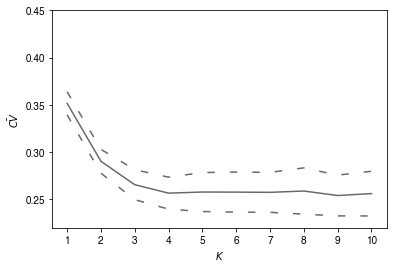
\includegraphics[scale=.5]{./Figures/cv_2.png}}
\end{minipage}%
\begin{minipage}{.5\linewidth}
\centering
\caption*{$\bar{CV}(p_{\hat{\theta}_{4,K}})$ for $K=1,\dots,10$}
\subfloat[]{\label{main:b}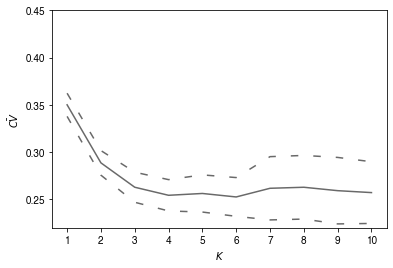
\includegraphics[scale=.5]{./Figures/cv_4.png}}
\end{minipage}%\par\medskip
\centering
\caption*{$\bar{CV}(p_{\hat{\theta}_{5,K}})$ for $K=1,\dots,10$}
\subfloat[]{\label{main:c}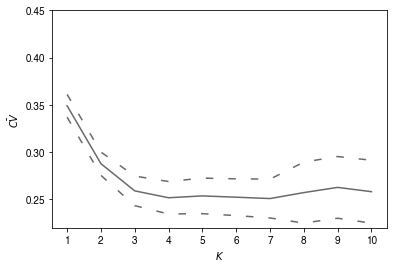
\includegraphics[scale=.5]{./Figures/cv_5.png}}

\footnotesize
  \textit{Note: In all plots the solid line is the average negative log likelihood averaged over the 5 estimates in the cross validation procedure for the finite mixture model with $K$ types. The dashed line is +/- one standard error of this estimate.}
\end{figure}

\begin{table}[!ht]
\caption{ML benchmarks on the heterogeneous level}
\label{tab:ML-het}
\centering
\begin{threeparttable}
\renewcommand{\TPTminimum}{\linewidth}
\begin{footnotesize}
\makebox[\linewidth]{%
\begin{tabular}{@{}lcc@{}}
\toprule
\toprule
     Model                          & $\bar{CV}(\cdot)$ & $\hat{e}(\ell(\cdot))$        \\ \midrule
$\hat{p}^*_{GB^{ind}}$                         & 0.3165       & 0.3081               \\
                       &   (0.0159)   &                      \\
$\hat{p}^*_{GB^{km}}$           & 0.2344       & 0.2305               \\
                      & (0.0143)     &                      \\
$\hat{p}^*_{GB^{hc}}$      & 0.2698       & 0.2434               \\
                       & (0.0105)     & \multicolumn{1}{l}{} \\
$\hat{p}^*_{GB^{ber}}$      & 0.2563       & 0.2363               \\
                       & (0.0180)     & \multicolumn{1}{l}{} \\ \midrule
\multicolumn{3}{l}{Number of subjects: 174}      \\
\multicolumn{3}{l}{Number of observations: 20,358}      \\ \bottomrule\bottomrule
\end{tabular}}
\end{footnotesize}
\begin{tablenotes}
      \footnotesize
      \item Note: $\hat{e}(\ell(\cdot))$ is the average negative log likelihood on the test set of the model. $\bar{CV}(\cdot)$ is the average negative log likelihood of the model with its optimal hyperparameters averaged over the five CV folds.  Standard error of the cross validation estimation in parentheses.
    \end{tablenotes}
\end{threeparttable}
\end{table}
\end{document}
